% vim: spelllang=en_gb

\documentclass[12pt,a4paper,draft]{scrartcl}
\usepackage{ifdraft}

% --------------------
% Set Language Options
% --------------------

\usepackage[nswissgerman,french,main=english]{babel}
\usepackage[autostyle,english=american,german=swiss]{csquotes}
\MakeOuterQuote{"}

\usepackage[shortcuts]{extdash}

% --------------
% Font & Symbols
% --------------

\usepackage{amssymb,mathtools}
\usepackage[warnings-off={mathtools-colon,mathtools-overbracket}]{unicode-math}
\usepackage[oldstyle,proportional]{libertinus-otf}

% ---------------
% Set Page Layout
% ---------------

% Get length of 65 characters
%\setlxvchars

\usepackage[driver=auto]{geometry}
% A5: 148mm × 210mm
% A4: 210mm × 297mm
\geometry{
  width=140mm,
  height=217mm,
  marginparsep=3mm,
  marginparwidth=30mm,
}
\ifdraft{\geometry{
  inner=10mm,
  marginparwidth=50mm
}}{}


% ---------------------
% Load Various Packages
% ---------------------

% Various Math Environments
\usepackage{amsthm,thmtools}
\usepackage{physics} % various shortcuts

% Bibliography
\usepackage{biblatex}
\addbibresource{bibliography.bib}

% For general figures
\usepackage[final]{graphicx}
\graphicspath{{/img}}
\usepackage{subcaption}
\usepackage{tikz}
\usetikzlibrary{babel,cd,shapes,3d}
\tikzcdset{arrow style=math font}
\tikzset{cross/.style={
    cross out, draw, solid, thin, 
    minimum size=2*(#1-\pgflinewidth), 
    inner sep=0pt, outer sep=0pt
  },
  cross/.default={3},
  conic/.pic={
    \begin{scope}[canvas is xz plane at y=0]
      \draw (0,0) circle [radius=0.5];
    \end{scope}
    \begin{scope}[canvas is xz plane at y=1]
      \draw (0,0) circle [radius=0.8];
    \end{scope}
    \begin{scope}[canvas is xz plane at y=-1]
      \draw (-20:.8) arc [start angle=-20,end angle=160,radius=.8];
      \draw[dotted] (160:.8) arc [start angle=160,end angle=340,radius=.8];
    \end{scope}
    \begin{scope}[rotate around y=20]
      \draw (.8,1) .. controls +(0,0) and +(0,.3) .. (0.5,0) .. controls +(0,-0.3) and +(0,0) .. (.8,-1);
      \draw (-.8,1) .. controls +(0,0) and +(0,.3) .. (-0.5,0) .. controls +(0,-0.3) and +(0,0) .. (-.8,-1);
    \end{scope}
  },
  degenerate conic/.pic={
    \begin{scope}[canvas is xz plane at y=1]
      \draw (0,0) circle [radius=.8];
    \end{scope}
    \begin{scope}[canvas is xz plane at y=-1]
      \draw (-20:.8) arc [start angle=-20,end angle=160,radius=.8];
      \draw[dotted] (160:.8) arc [start angle=160,end angle=340,radius=.8];
    \end{scope}
    \begin{scope}[rotate around y=20]
      \draw (-.8,-1) -- (.8,1);
      \draw (-.8,1) -- (.8,-1);
    \end{scope}
  },
  reduced conic/.pic={
    \begin{scope}[canvas is xz plane at y=1]
      \draw[very thin, opacity=0.5] (0,0) circle [radius=.8];
      \draw (-32:.8) arc [start angle=-32,end angle=32,radius=.8];
    \end{scope}
    \begin{scope}[canvas is xz plane at y=-1]
      \draw[very thin, opacity=0.5] (0,0) circle [radius=.8];
      \draw (-32:.8) arc [start angle=-32,end angle=32,radius=.8];
    \end{scope}
    \begin{scope}[canvas is xz plane at y=0]
      \draw[very thin, opacity=0.5] (0,0) circle [radius=.5];
      \draw (-32:.5) arc [start angle=-32,end angle=32,radius=.5];
    \end{scope}
    \foreach \φ in {32,-32} {
      \begin{scope}[rotate around y=\φ]
        \draw (.8,1) .. controls +(0,0) and +(0,.3) .. (0.5,0) .. controls +(0,-0.3) and +(0,0) .. (.8,-1);
      \end{scope}
    }
    \begin{scope}[rotate around y=20]
      \draw[very thin, opacity=0.5] (-.8,1) .. controls +(0,0) and +(0,.3) .. (-0.5,0) .. controls +(0,-0.3) and +(0,0) .. (-.8,-1);
    \end{scope}
  }
}

% For lists
\usepackage[shortlabels]{enumitem}

% For better Tables
\usepackage{tabularray}

% For more fine grained typesetting in final mode.
% Else set the tolerance for overfull warnings higher.
\ifdraft{\hfuzz=1.5pt}{\usepackage{microtype}}

% Links and stuff
\usepackage[final]{hyperref}
\usepackage[noabbrev,capitalize]{cleveref}

% For Todonotes
\usepackage[obeyDraft]{luatodonotes}

% --------------------------------------------
% Define Theorem Environments & Math Operators
% --------------------------------------------

\declaretheorem[numberwithin=section]{theorem}
\declaretheorem[sibling=theorem]{lemma, proposition, corollary}
\declaretheorem[sibling=theorem,style=definition]{definition, example}
\declaretheorem[sibling=theorem,style=remark]{remark}

\DeclareMathOperator{\id}{id}
\DeclareMathOperator{\im}{im}
\DeclareMathOperator{\Aut}{Aut}
\DeclareMathOperator{\Diff}{Diff}
\DeclareMathOperator{\GL}{GL}
\DeclareMathOperator{\HF}{HF}
\DeclareMathOperator{\HM}{HM}
\DeclareMathOperator{\Hom}{Hom}
\DeclareMathOperator{\Ext}{Ext}
\DeclareMathOperator{\Tor}{Tor}
\DeclareMathOperator{\Flux}{Flux}
\DeclareMathOperator{\Crit}{Crit}

\begin{document}
\title{Semi-Local Lagrangian Tori in Dimension Four}
\author{JoJoJo}

\maketitle

\section{Introduction}

\section{Local model}

We use almost toric geometry to define the local model spaces. In Sections \ref{sec:atgeometry},\ref{sec:atfibres}, we give a short overview of almost toric geometry, its basic operations (nodal trades, nodal slides, mutations) and its fibres. The reader familiar with the ATF-framework can skip this section. In ... we ...


\subsection{Almost toric fibrations and their base diagrams}
\label{sec:atgeometry}

Almost toric geometry is a generalization in dimension four of toric geometry. Let us briefly discuss the latter, before moving to the almost toric case. A symplectic toric four-manifold $(X,\omega,\mu)$ is a symplectic manifold $(X,\omega)$ equipped with a moment map $\mu \colon X \rightarrow \mathbb{R}^2$ generating an effective Hamiltonian $T^2$-action on $X$. The image $\mu(X) = \Delta \subset \mathbb{R}^2$ is a so called Delzant polytope and classifies $(X,\omega)$ up to $T^2$-equivariant symplectomorphisms, see \cite{Del88} or \cite{Can03} for more details. The moment map defines a Lagrangian torus fibration, or, equivalently\footnote{we use both terms interchangeably}, a completely integrable system on $X$. The Lagrangian torus fibration defined by a toric moment map has very special properties, namely (1) its singularities (located over the boundary of $\Delta$) are of elliptic-regular or of elliptic-elliptic type, and (2) the moment map defines action coordinates on the interior of the moment polytope. Note that every Lagrangian torus fibration admits local action coordinates in the neighbourhood of a regular fibre (this is the classical Arnold-Liouville Theorem), but that these do not necessarily extend globally, see for example \cite{Dui80} or \cite{Zun96,Zun03}.

An \textbf{almost toric fibration (ATF)} is a Lagrangian torus fibration on a four-dimensional symplectic manifold whose singularities are all of elliptic-regular, elliptic-elliptic or focus-focus type. Almost toric fibrations were introduced by Symington \cite{symington2002FourDF}, based on earlier work by Zung \cite{Zun96,Zun97,Zun03}. As opposed to toric manifolds, there is no globally defined Hamiltonian torus action at play, nor is there a moment map. The analogue of the moment map image is given by the so-called \textbf{almost toric base diagram}. As in the case of Delzant polytopes, every almost toric base diagram defines a unique symplectic manifold, see \cite[Corollary 5.4]{symington2002FourDF} \cite[Theorem 8.5]{evans2021atfs}. 

For us\footnote{The general almost toric framework allows for much more generality, e.g. base diagrams carrying topology, non-convexity etc. but for our purposes the description we give here is sufficient.}, the almost toric base diagram is given by a rational convex polytope $\Delta \subset \mathbb{R}^2$ in the plane decorated with nodes and branch cuts\footnote{By a small abuse of notation, we denote by the symbol $\Delta$ the almost toric base diagram, as well as the subset $\Delta \subset \mathbb{R}^2$ (without decorations).}. Given an almost toric fibration $F \colon X \rightarrow B \subset \mathbb{R}^2$, the corresponding base diagram is computed, roughly speaking, by attempting to find global action coordinates on the locus of regular values of $F$ in the base $B$. In the absence of focus-focus singularities (i.e. in the toric case), this succeeds, the action coordinates can be extended over the elliptic-type singularities and this procedure yields the moment map. However in the presence of focus-focus singularities, this fails. Indeed, a neighbourhood of a focus-focus singularity (whose image sits in the interior of $\im F$) carries topological monodromy, meaning that the torus bundle given by neighbouring regular fibres is non-trivial. See e.g.\ \cite{Zun97} for more details. This means that action coordinates are well-defined only on the universal cover of $B \setminus \{nodes\}$. An almost toric base diagram is obtained by computing action coordinates on a fundamental domain in the universal cover, see \cite[Definition 8.3]{evans2021atfs} for more details. The branch cut decorations (represented by dashed lines) of the almost toric base diagram indicate which choice of fundamental domain was made. Equivalently, one can think of the branch cuts as curves which were removed from the regular locus of $F$ in $B$ in order to make it simply connected. On a simply connected domain, one can compute unique (up to the usual action of $\operatorname{GL}(2;\mathbb{Z}) \ltimes \mathbb{R}^2$) action coordinates. The image of these action coordinates yields the interior of the almost toric base diagram. The full base diagram is obtained after adding the following decorations: edges and vertices on the boundary represent elliptic-type singularities (as in the toric case), dashed lines represent the image of the branch cuts in action coordinates and crosses represent nodes, i.e.\ fibres containing a focus-focus singularity. As mentioned above, a fully decorated almost toric base diagram, defines a unique symplectic manifold.

In this paper, we will always make a special choice of almost toric base diagram. Every node in the almost toric base diagram has a unique \textbf{eigendirection}, i.e. a direction in $\mathbb{R}^2$ yielding an action coordinate which is preserved under the monodromy of the given node. Equivalently, there is a subcircle of the nearby regular tori whose Hamiltonian $S^1$-action extends over the focus-focus singularity. Although the eigendirection is not explicitely part of the decorations of the almost toric base diagram, it can always be read off from the angle the branch cut forms at the node in question. In the current paper, we always choose the branch cut to coincide with the eigendirection. As a consequence, the almost toric base diagram "closes up" (we refer to the discussion in \cite[7.2]{evans2021atfs}) and thus yields a convex polytope. With this convention, there is an analogue of the moment map, given by a continuous map $\pi \colon X \rightarrow \Delta$, which we call \textbf{almost toric moment map}\footnote{This is non-standard terminology}. We give a brief outline on how to construct $\pi$. Let $\Delta_0 \subset \Delta$ be the complement of nodes and branch cuts. Since $\Delta_0$ is simply connected, there are global action coordinates on its intersection with the regular locus, see \cite{Dui80}. Away from the branch cut and nodes, all singularities are of toric type (i.e.\ elliptic-regular or elliptic-elliptic), meaning that the map given by action coordinates can be smoothly extended over the singularities to yield a moment map $\pi\vert_{X_0} \colon X_0 \rightarrow \Delta_0$ of a Hamiltonian $T^2$-action. With our choice of branch cuts, this map has a continuous extension $\pi \colon X \rightarrow \Delta$. Let us formulate the following statement for future reference. 

\begin{proposition}
    \label{thm:toricmomentmap}
    The restriction $\pi\vert_{X_0} \colon X_0 = \pi^{-1}(\Delta_0) \rightarrow \Delta_0$ is a toric moment map. 
\end{proposition}



Then $\pi$ has the property that its restriction $\pi\vert_{X_0} \colon X_0 = \pi^{-1}(\Delta_0) \rightarrow \Delta_0$ is an honest toric moment map. Roughly speaking, the almost toric moment map is obtained by picking action coordinates on $X_0$ (this is possible since it fibers over the simply-connected $\Delta_0$) and by (continuous) extension over the branch cuts. \\

One of the main features of almost toric geometry is that, one can deform a given (almost) toric fibration $F \colon X \rightarrow \mathbb{R}^2$ to produce another one on the same symplectic manifold $X$. This freedom distinguishes the almost toric from the classical toric case. The main two main operations by which one can deform an almost toric fibration are the nodal trade and the nodal slide, both of which can be handily represented by simple operations on the corresponding ATF-base diagrams. Let us briefly discuss these operations, referring to \cite[Sections 8.2-8.3]{evans2021atfs} for details. The \textbf{nodal trade} takes an elliptic-elliptic singularity and transforms it into a focus-focus singularity, while merging the two families of elliptic-regular singularities into one. In terms of the almost toric base diagram, it corresponds to replacing toric vertex with a node and a branch cut. The \textbf{nodal slide} consists of moving the focus-focus singularity in a non-trivial way (in terms of action coordinates) such that the node in the base diagram moves on a line in its eigendirection. The third operation is called \textbf{changing the branch cut}, see \cite[Sections 8.4]{evans2021atfs} for more details. It corresponds to making a different choice of branch cut to produce the almost toric base diagram. Since, in the context of the present paper, we only consider branch cuts which coincide with the Eigenline of a given node, there are only two choices of branch cuts and the \textit{change in branch cut}-operation is a switch from one to the other. Under such a switch, the almost toric base diagram undergoes a piece-wise linear transformation: apply the identity to one of the halves of the base diagram bounded by the eigenline and a integral shear preserving the eigenline to the other half. We refer to \cite[Example 8.15]{evans2021atfs} for an example. Note that there is a difference between nodal trade and nodal slide on one hand, and the change in branch cut operation on the other hand. The first two operations represent a change in the underlying almost toric fibration on $X$, whereas the change in branch cut does not. The change in branch cut merely corresponds to a different way of representing the almost toric fibration by a base diagram.

Together, these three operations add up to an easy-to-use visual calculus on almost toric base diagrams, all of which represent different almost toric fibrations on the same manifold. The combination of nodal slides and changes in branch cut is often called a \textbf{mutation}. For example, one can start with a toric manifold, apply nodal trades at its vertices and then perform a series of mutations. This was used in symplectic topology to great effect by Vianna~\cite{Via16} to exhibit infinitely many almost toric fibrations on $\mathbb{C}P^2$. The set of almost toric fibrations obtained in this way is in bijection with the set of Markov triples and each almost toric fibration has an exotic Lagrangian torus as monotone fibre.

\subsection{Almost toric fibres}
\label{sec:atfibres}

Let $F \colon X \rightarrow B \subset \mathbb{R}^2$ be an almost toric fibration with ATF-base diagram $\Delta$. A fibre of $F$ is called \textbf{almost toric fibre}. For every $x \in \Delta$, we denote by $T(x) \subset X$ the unique set in $X$ whose action coordinates are equal to $x$ with the chosen branch cuts. Recall that, in the context of this paper, there is an almost toric moment map $\pi \colon X \rightarrow \Delta$ and thus we have $T(x) = \pi^{-1}(x)$. If $x \in \partial \Delta$, then $T(x)$ is a point or an isotropic circle. If $x$ is a node, then $T(x)$ is a Lagrangian Whitney sphere, i.e.\ a Lagrangian immersion of a $2$-sphere with one transverse self-intersection. If $x$ is neither a node, nor contained in the boundary, then $T(x)$ is a Lagrangian torus and we call such a torus a \textbf{regular ATF-fibre}.

\begin{remark}
    \label{rk:pinchedtorus}
    A Lagrangian Whitney sphere living over the node of an ATF-base diagram can be interpreted as a limit of regular fibres (i.e.\ Lagrangian tori) by viewing it as a Lagrangian torus which is "pinched" along a curve on the torus. The homology class of this curve determines determines the topological monodromy of the torus bundle in a neighbourhood of the node.
\end{remark}

Almost toric fibres are left unaffected by nodal slides, provided they are not contained in the segment on which the nodal slide is supported\footnote{By this we mean the line segment obtained as the union of points across which the node moves during the nodal slide.}.

\begin{lemma}
    \label{thm:nodal_slide}
    Let $\Delta, \Delta'$ be two almost toric base diagrams which are related by nodal slides\footnote{This impies that the underlying sets $\Delta, \Delta' \subset \mathbb{R}^2$ coincide.} that are supported in the set $\Sigma$. Let $X,X'$ be symplectic manifolds corresponding to $\Delta,\Delta'$ and dentote by $T(x) \subset X$ and $T'(x) \subset X$ their respective ATF fibres. Then for every $x \in \Delta \setminus \Sigma$, there is a symplectomorphism $\psi \colon X \rightarrow X'$ with $\psi(T(x)) = T'(x)$.\todo{(definition nodal slide) und bild dazu.}
\end{lemma}

\begin{proof}
    This follows from the proof of \cite[Theorem 8.10]{evans2021atfs}, by taking the set $K \subset \Delta$ therein small enough so that $x \notin K$.
\end{proof}

\begin{remark}
    \label{rk:slides_ray}
    The claim of \cref{thm:nodal_slide} fails for points which are contained in a segment on which a nodal slide is supported, even if both points correspond to regular almost toric fibres. In fact, this is one of the main sources to construct so-called exotic Lagrangian tori, i.e.\ sets of tori for which there is no ambient symplectomorphism mapping one to the other. This approach was pioneered by Vianna \cite{Via16,Via17}. The simplest example in which this occurs is $\mathbb{R}^4 = \mathbb{C}^2$. Let $T_{\text Cl}(a) = S^1(a) \times S^1(a) \subset \mathbb{C} \times \mathbb{C}$ be the Clifford torus. It is the toric fibre over the base point $(a,a)$ in the standard toric structure on $\mathbb{R}^4$. To obtain an almost toric fibration with one focus-focus singularity on $\mathbb{R}^4$, perform a nodal trade at the vertex of the toric structure. By a nodal slide, move the node across $(a,a)$ to obtain the Chekanov torus $T_{\text Ch}(a)$ over the point $(a,a)$.
\end{remark}



\subsection{Model spaces}

Let $d,p,q \in \mathbb{N}$ be integers such that $d≥1$,   $p,q$ are coprime\footnote{Here, we consider the pair $(1,0)$ as coprime.} and with $p>q≥0$. Let $\Delta_{dpq}$ be the almost toric base diagram obtained by decorating the right half-plane
$$\Delta_{dpq} = \{ (x,y) \in \mathbb{R}^2 \, \vert \, x \geqslant 0 \}$$
with $d$ distinct nodes contained in the ray,
\begin{equation}
  \label{eqn:eigenline}
  R = \{\alpha (p,q) \in \Delta_{dpq} \, \vert \, \alpha > 0 \}
\end{equation}
and with eigendirection $(p,q)$. For a branch cut contained in $R$ and to the right of the nodes, this yields the almost toric base diagram depicted in \cref{fig:Bdpq_moment_image}(a). 

\begin{definition}
    \label{def:bdpq}
    Let $B_{dpq}$ be the symplectic manifold having $\Delta_{dpq}$ as almost toric base diagram. 
\end{definition}

Such a symplectic manifolds exists, see \cite[Section 7.4]{evans2021atfs} and is thus unique by \cite[Theorem 8.5]{evans2021atfs}. 

\begin{remark}
    The symplectic manifold $(B_{dpq}, \omega)$ is exact. Indeed, we will see in \cref{sec:homology} that there is a set of generators of $H_2(B_{dpq})$ represented by Lagrangian spheres, meaning that $[\omega] = 0 \in H^2(B_{dpq};\mathbb{R})$. The space $B_{dpq}$ can be realized as the Milnor fibre of a smoothing of certain cyclic quotient singularities. For more details on this, see \cite[Section 7.4]{evans2021atfs} or \cite{Eva19}.
\end{remark}

Note that $\Delta_{dpq}$ depends on $d$ parameters $n_1,\ldots,n_d > 0$ which correspond to the $x$-coordinate of the position of the nodes. The symplectic manifold in \cref{def:bdpq} is independent of the position of the nodes, which is why we suppress the dependency on the $n_i$ in the notation. Indeed, any configuration of $d$ nodes on a common eigenline is related to any other such configuration by nodal slide. By \cite[Theorem 8.10]{evans2021atfs}, this means that the space $B_{dpq}$ is well-defined up to symplectomorphism.

We turn to the almost toric fibres of $B_{dpq}$. For every $x \notin R$, we denote the corresponding almost toric fibre by $T(x) \subset B_{dpq}$. This definition is independent of the position of the nodes in $\Delta_{dpq}$ by \cref{thm:nodal_slide}. In case $x \in R$, the definition depends on how many nodes are to the right and to the left of $x$. For every $a > 0$, let $x_a = \left( a,\frac{aq}{p} \right) \in R$. For every $k \in \{0,\ldots,d\}$, let $\Delta_{dpq}$ be an almost toric base diagram as above for which $k$ of the $d$ nodes are to the left of the point $x_a$. 

\begin{definition}
    Let $a>0$ and $k \in \{0,\ldots,d\}$. We denote by $T^k_{pq}(a) = T(x_a)$ the regular almost toric fibre of a fibration whose almost toric base diagram has $k$ of the $d$ nodes to the left of $x_a$. 
\end{definition}

Again, by \cref{thm:nodal_slide}, this definition does not depend on the precise position of the nodes, only on $k$, i.e.\ the number of nodes to the left of $x_a$. In ..., we show that there is no symplectomorphism of $B_{dpq}$ mapping $T^k_{pq}(a)$ to $T^{k'}_{pq}(a)$ if $k \neq k'$.


\subsection{Some symplectic embeddings}
\label{ssec:sembeddings}

Let $X = \mathbb{R} \times T^*S^1$ be the symplectic manifold equipped with the product symplectic form $\omega_{\mathbb{C}} \oplus \omega_{T^*S^1}$ equipped with the toric structure defined by the moment map
\begin{align*}
    μ_0 \colon ℂ × T^* S^1 &→ \Delta_0 = \{x ∈ ℝ² \mid x_1 ≥ 0\}\\
    (z,p,θ) &↦ (\pi \abs{z}^2, p) \; . 
\end{align*}

For every $x \in \operatorname{int} \Delta_0$, we denote the corresponding toric fibre by $T_0(x) = \mu_0^{-1}(x) \subset X$. Note that, up to the $d$ nodes, the almost toric base diagram $\Delta_{dpq}$ discussed in \cref{sec:atgeometry} agrees with $\Delta_0$. This leads to the following

\begin{lemma}
    \label{thm:sembedding}
    Let $A \subset \Delta_0$ be a subset contained in a compact subset. Then there is a symplectic embedding $\psi \colon \mu_0^{-1}(A) \hookrightarrow B_{dpq}$ with\footnote{By $T_{dpq}^{(0)}(x)$, we mean $T_{dpq}^0(x)$ if $x \in R$ and $T_{dpq}(x)$ if not. See \cref{def:bdpqfibres}.} $\psi(T_0(x)) = T_{dpq}^{(0)}(x)$ for all $x \in A$.
\end{lemma}

\begin{proof}
    Since $\Delta_{dpq}$ and $\Delta_0$ agree as sets (i.e.\ ignoring almost toric decorations), we can view $A$ as a subset of $\Delta_{dpq}$. Since $A$ is contained in a compact subset, we can assume, by \cref{thm:nodal_slide}, that all nodes and Eigenrays of the ATF base diagram $\Delta_{dpq}$ of $B_{dpq}$ are disjoint from $A \subset \Delta_{dpq}$. On the complement of the nodes and their eigenrays, the almost toric moment map $\pi \colon B_{dpq} \rightarrow \Delta_{dpq}$ restricts to an honest toric moment map, see \cref{rk:atfbasediagram}. Since toric manifolds are classified up to fibre-preserving symplectomorphisms by the image of their moment map, there is a symplectomorphism $\psi$ mapping $\mu_0^{-1}(A)$ to $\pi^{-1}(A) \subset \Delta_{dpq}$ which satisfies $\psi(T_0(x)) = T_{dpq}^{(0)}(x)$ for all $x \in A$.
\end{proof}



\subsection{Homology of \texorpdfstring{$B_{dpq}$}{Bdpq}}
\label{sec:homology}

Let $T(x) = π^{-1}(x) \subset B_{dpq}$ for $x ∈ Δ_{dpq}$ be a regular almost toric fibre. In the computation of the displacement energy of $T(x)$, we rely on an explicit basis of the relative homology group $H_2\qty(B_{dpq},T(x))$.

\begin{lemma}
  \label{thm:homology}
  We have
  \begin{align*}
    H_0(B_{dpq}) &≅ ℤ & H_1(B_{dpq}) &≅ ℤ_p & H_2(B_{dpq}) &≅ ℤ^{d-1} \\
                 &    &              &      & H_2(B_{dpq},T(x)) &≅ ℤ^{d+1}
  \end{align*}
\end{lemma}

\begin{proof}
    Here we follow very closely \cite[Lemma 7.11]{evans2021atfs}, but we additionally calculate the the relative second homology group. Since all $T(x) = π^{-1}(x)$ are homotopic, we may assume that $x = (x_1,x_2)$ is on the ray $R$ (see \eqref{eqn:eigenline}), such that all the nodes are to the right of $x$ as in \cref{fig:branch_cut_retraction}.

    As in \cite[Lemma 7.11]{evans2021atfs}, $B_{dpq}$ retracts onto $π^{-1}(ℓ)$, where $ℓ ⊂ R$ is a closed line segment containing $0, x$ and all the nodes (See \cref{fig:branch_cut_retraction} again).
    We investigate the topology of the preimage $π^{-1}(ℓ)$ in two steps. If there were no nodes on the line, the preimage is a solid torus, denoted by $\hat{T}$, with boundary $∂ \hat{T}$ homotopy equivalent to $T(x)$. 
    If there are nodes on the line $ℓ$, then the singular fibres play a role in the calculation of the homology groups as follows. In the basis of $H₁(∂ \hat{T})$, derived from the action coordinates defined away from the branch cut, such that for each critical fibre $k ∈ \qty{1,…,d}$ we collapse a loop representing the homology class $(-q,p) \in H₁(∂ \hat{T})$, as in \cref{fig:collapse_cycles}.\footnote{In this basis the class $(1,0)\in H_1(\partial \hat{T})$ corresponds to the class that bounds a disk in $\hat{T}$ and $(1,0)\in H_1(\partial \hat{T})$ is the class that is homotopic to the core circle of $\hat{T}$.}

    Up to homotopy this is the same as attaching a disk $D_k$ along $(-q,p)$.
    Furthermore, up to homotopy we can also require that the $d$ discs $D_1,…,D_d$ are attached along $∂ \hat{T}$.
    Denote the resulting space by $S$, which is a solid torus $\hat{T}$ with the disks $D_i$ attached.

\begin{figure}
  \centering
  \begin{subfigure}{0.45\textwidth}
    \centering
    \begin{tikzpicture}
      \fill[opacity=0.2] (0,3) rectangle (6,-1);
      \draw[thick] (0,3) -- (0,-1);
      \draw[line width=0.08cm,red,opacity=0.4,text opacity=1] (0,0) -- node[pos=0.75, anchor=north] {$ℓ$} (4,2);
    \fill (1,0.5)  circle[radius=1pt] node[anchor=south] {$T(x)$};
      \draw[dashed] (2,1) node[cross] {} -- (4,2) node[cross] {} -- (6,3);
    \end{tikzpicture}
    \caption{Retraction to branch cut line}
    \label{fig:branch_cut_retraction}
  \end{subfigure}%
  \begin{subfigure}{0.55\textwidth}
    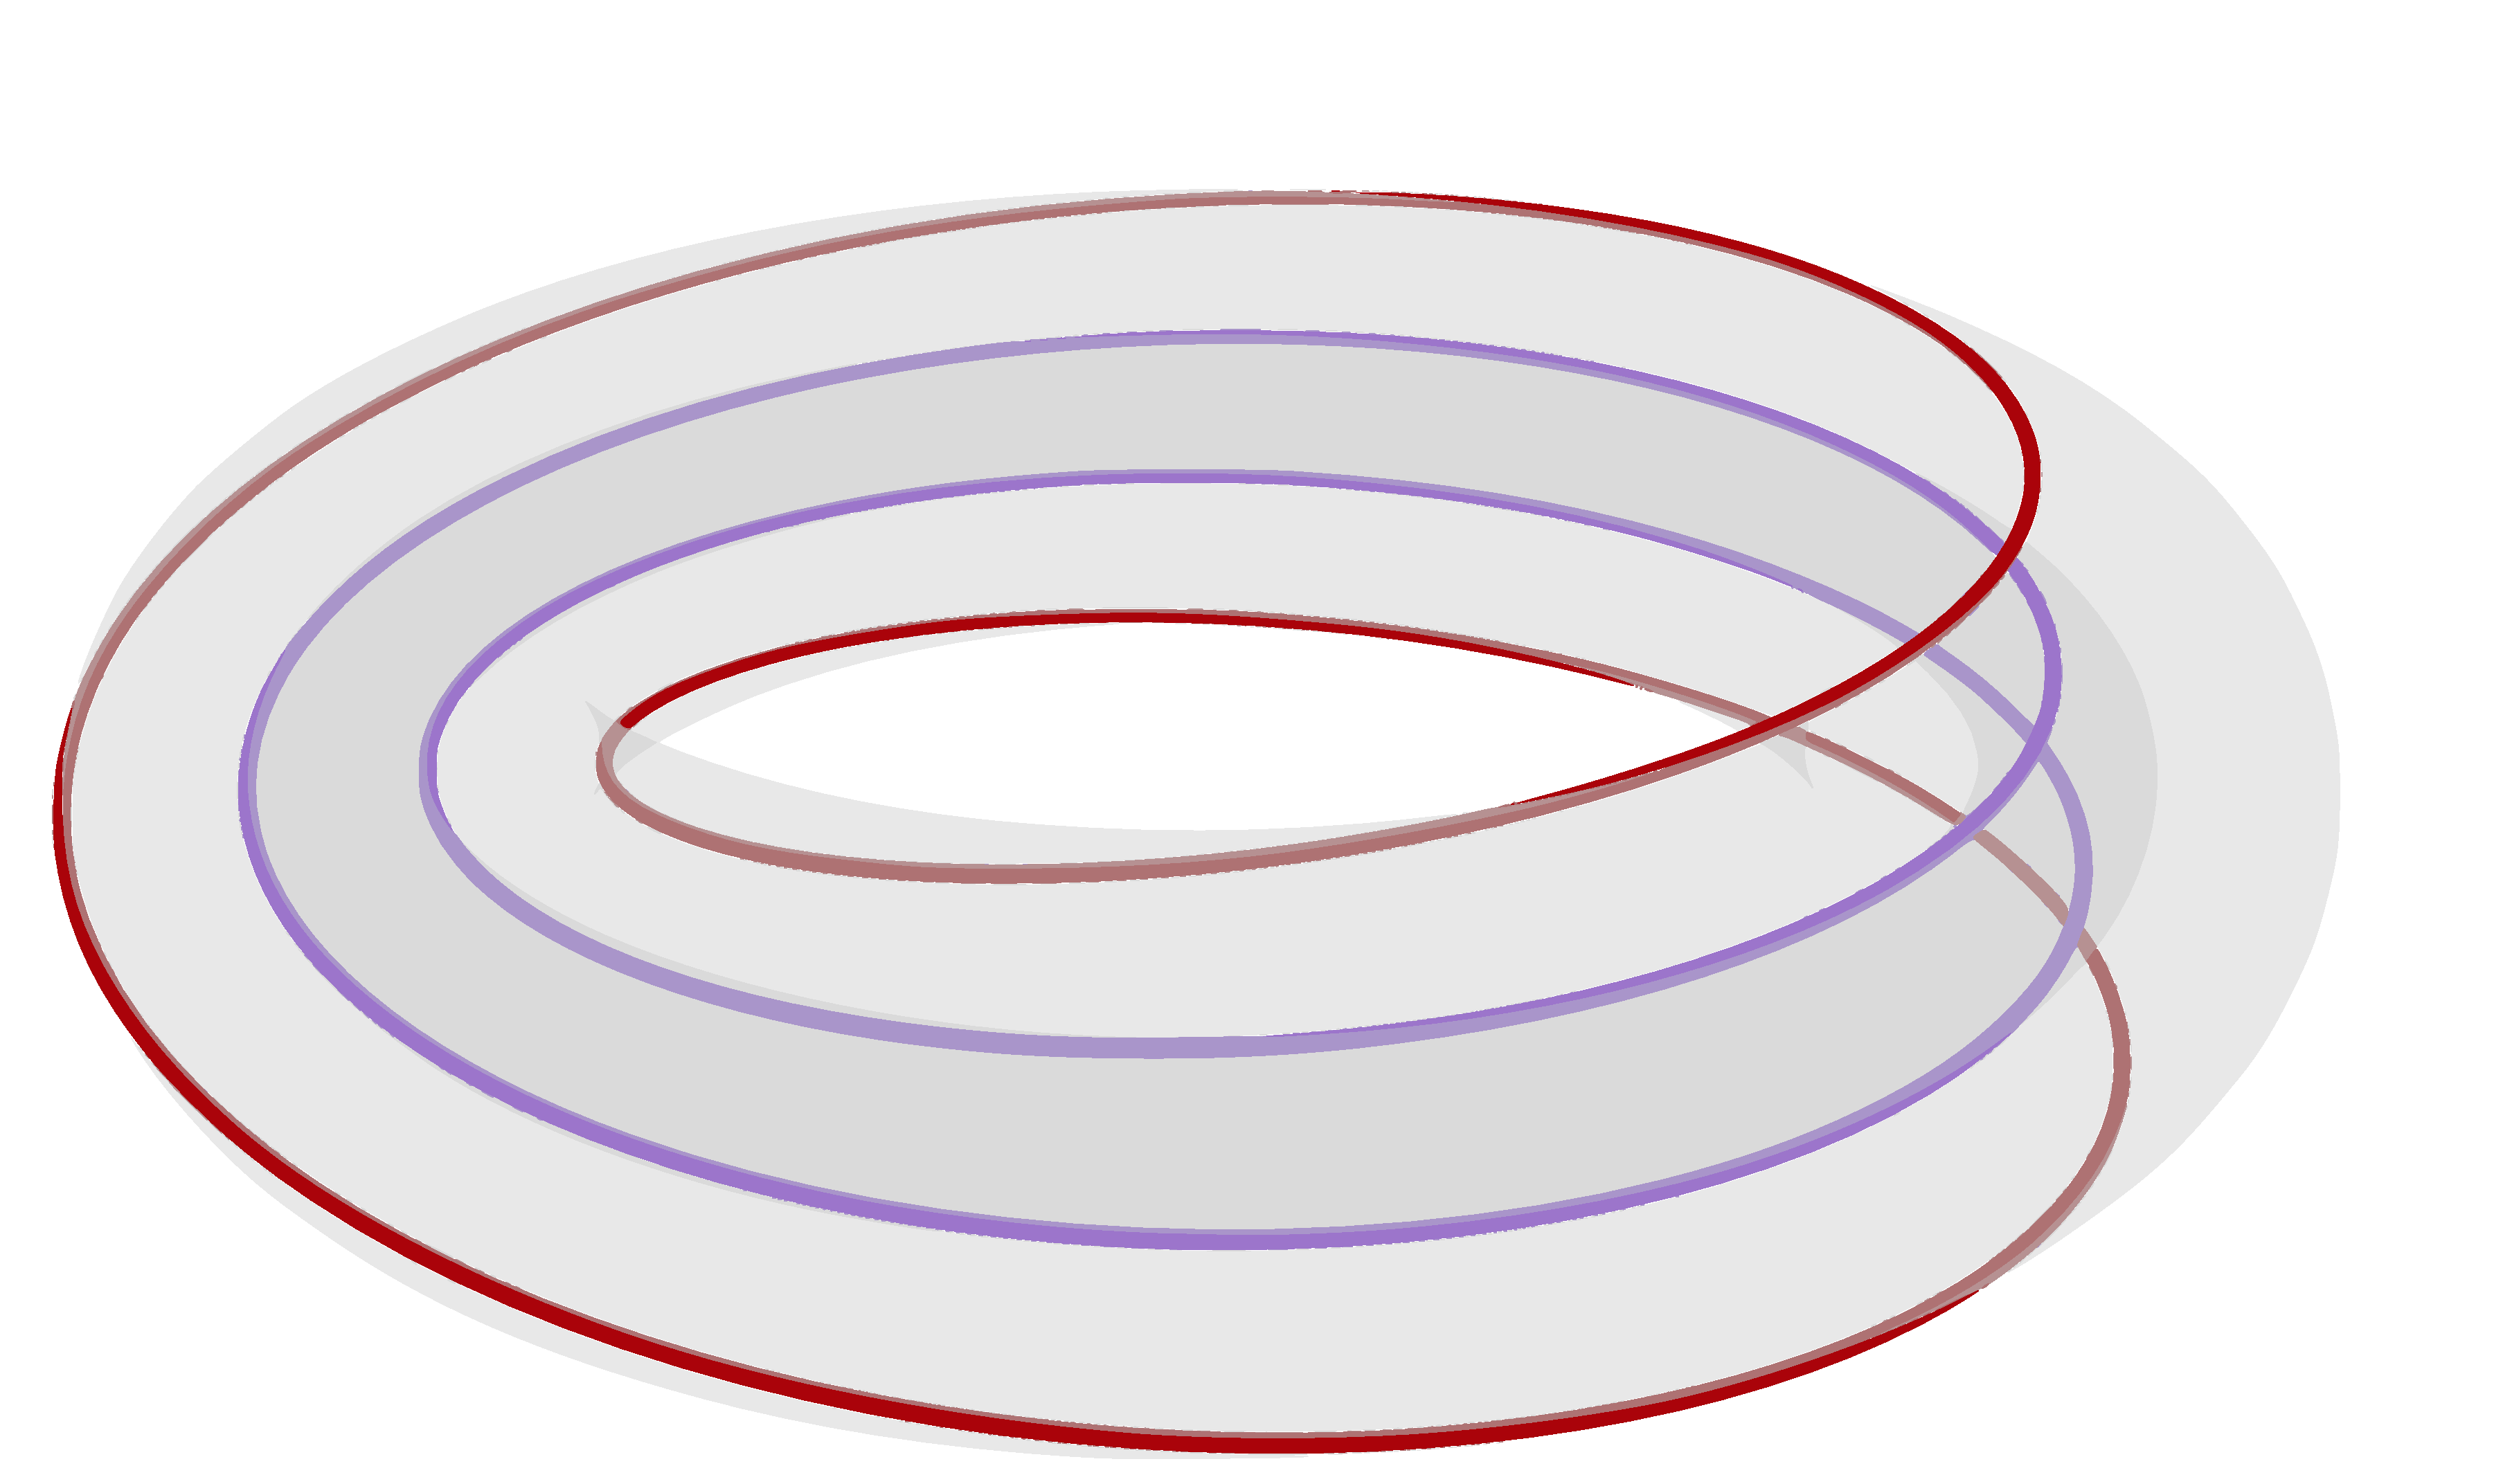
\includegraphics[width=\textwidth]{img/homology_collapse.pdf}
    \caption{The two cycles marked in red and purple (here $p=2, q=1$) are collapsed to a point.}
    \label{fig:collapse_cycles}
  \end{subfigure}
  \caption{Calculation of the homology of $B_{dpq}$}
\end{figure}

Consider the long exact sequence of homology for the pair $(S,∂ \hat{T})$:

\[
\begin{tikzcd}[column sep=small]
  H_2(∂ \hat{T}) \ar[r,"0"] &
  H_2(S) \ar[r,hook]\ar[d,"≅"] &
  H_2(S,∂ \hat{T}) \ar[r]\ar[d,"≅"] &
  H_1(∂ \hat{T}) \ar[r,two heads]\ar[d,"≅"] &
  H_1(S) \ar[r,"0"] \ar[d,"≅"] &
  H_1(S, ∂ \hat{T}) \ar[d,"≅"]
  \\
  &
  ℤ^{d-1} &
  ℤ^{d+1} &
  ℤ² &
  ℤ_p &
  0
\end{tikzcd}
\]

The first horizontal map is trivial, since $∂ \hat{T}$ is homotopic to the core circle in $S$.

The homology $H_2(S)$ can be calculated by contracting the solid torus $\hat{T}$ in $S$ onto the core circle. Therefore, we see that $S$ is homotopic to a circle with $d$ discs glued to its boundary by a degree $p$ map. Hence, $H_2(S)$ is generated by the visible Lagrangian spheres $\qty{S_2,…,S_d}$ mentioned in \cref{rem:B_dpq_skeleton}, since $[S_k] = [D_{k-1}]-[D_k]$.

$H_2(S,∂ \hat{T})$ is generated by the discs $D_0,…,D_d$, where $D_0$ is given by a disc that retracts onto a point on the "core" circle of $S$. These discs can be seen schematically in \cref{fig:homology_generating_discs}, where the disc $D_0$ intersecting the toric boundary collapses the $(0,1)$ cycle in the toric fibre $T(x)$ and the discs intersecting the critical points collapse the $(-q,p)$ cycle (see \cref{fig:homology_generating_discs}).

The boundary map $∂ \colon H_2(S,∂ \hat{T}) → H_1(∂ \hat{T})$ is given by $\partial D_0 = (0,1)$ and $\partial D_i = (-q,p)$, for $k ∈ \qty{1,…,d}$, meaning that the map $H_1(∂ \hat{T}) → H_1(S)$ maps $(0,1)$ to the generator of $ℤ_p$.
\end{proof}

\begin{figure}
  \centering
  \begin{tikzpicture}
    \fill[black!5] (0,4) rectangle (7,-1);

    \coordinate (xy) at (2.7,3.5);
    \node[anchor=south] at (xy) {$T(x)$};
    \fill (xy) circle[radius=.05];
    \draw (xy)
           .. controls +(0,0) and +(-.5,1) .. node[anchor=east, near end] {$D₁$} (2,1)
      (xy) .. controls +(0,0) and +(-.5,1) .. node[anchor=west, near end] {$D₂$} (4,2)
      (xy) .. controls +(0,0) and +(-.5,1) .. node[anchor=west, near end] {$D₃$} (6,3)
      (xy) .. controls +(0,0) and +(1,0) .. node[anchor=south, near end] {$D₀$} (0,2.5);

    \draw[ultra thick, blue, draw opacity=.3] (2,1) -- node[anchor=north] {$S₂$} (4,2);
    \draw[ultra thick, purple, draw opacity=.3] (4,2) -- node[anchor=north] {$S₃$} (6,3);

    \draw[thick,dotted] (2,1) node[cross] {} -- (4,2) node[cross] {} -- (6,3) node[cross] {} -- (7,3.5);

    \draw[thick] (0,4) -- (0,-1);
  \end{tikzpicture}

  \caption{The disks $D₀, …, D_d$ generating the homology $H₂\qty(B_{dpq}, T(x))$, presented schematically.}
  \label{fig:homology_generating_discs}
\end{figure}






\section{Versal Deformations \& Nearby Lagrangians}

Let $L_0 ⊂ (X,ω)$ be a compact Lagrangian, and $\overline{\symcal{L}}$ the space of Lagrangians in $X$ equipped with the $\symcal{C}^1$-topology.

\begin{definition}
  A \textbf{Lagrangian isotopy} is a map $\Lambda \colon [0,1] \rightarrow \overline{\symcal{L}}, t \mapsto \Lambda_t$ with $\Lambda_0 = L_0$ s.t.\ there is a smooth map $[0,1] \times L_0 \rightarrow X$ which maps $\{t\} \times L$ to $\Lambda_t$.

  Note that we can always find a smooth isotopy $φ_t \colon X → X$ s.t.\ $φ_t(L_0) = Λ_t$. We say that \textbf{$Λ$ is generated by $φ$}.
\end{definition}

By $\symcal{L}_{L_0} ⊂ \overline{\symcal{L}}$ (or simply $\symcal{L}$), denote the set of Lagrangians which are Lagrangian isotopic to $L_0$.
See \cite{ono2008LagrangianFlux} for more details on the $\symcal{C}^1$-topology on the space of Lagrangians.
Denote by $\tilde{\symcal{L}}$ the universal cover of $\symcal{L}$, that is the space of Lagrangian isotopies of $L_0$ up to endpoint preserving isotopies. Using Weinstein's Lagrangian neighbourhood theorem, one can check that $\symcal{L}$ is locally simply connected, showing that $\tilde{\symcal{L}} \rightarrow \symcal{L}$ is indeed the universal cover.

\begin{definition}
  \label{def:flux_map}
  Let $Λ \colon ([0,1],0) → (\symcal{L},L_0)$ be a Lagrangian isotopy. Its \textbf{(Lagrangian) flux} is the map
$$    H_1(L_0) → ℝ, \quad    ξ ↦  ∫_{C_ξ} ω, $$
where $C_ξ$ is the cylinder obtained by sliding a representative of $ξ$ in $L_0$ along the Lagrangian isotopy (called a \textbf{flux cylinder of $ξ$ over $Λ$}).
  This map is well defined (independent of the choice of $C_ξ$) and also independent by end point preserving isotopies of $Λ$.\footnote{If $C_ξ ≅ C_ξ'$ by homotopy $H$, $0=∫_{∂H} ω = ∫_{C_ξ} ω - ∫_{C_ξ'} ω + ∫_A ω + ∫_B ω$, with $A,B$ contained in the endpoints of the isotopy, which are Lagrangian.}

  Using $\Hom(H_1(L_0),ℝ) = H^1(L_0;ℝ)$ this gives a well defined map
  \[ \Flux \colon \tilde{\symcal{L}} → H^1(L_0;ℝ) \; ,\]
  called the \textbf{flux map}.
\end{definition}

\begin{lemma}
  \label{thm:hamiltonian_flux}
  A Lagrangian isotopy $Λ$ is generated by a Hamiltonian isotopy, iff $∀t ∈ [0,1], \Flux(Λ_s|_{s ∈ [0,t]}) = 0$.
\end{lemma}
\begin{proof}
  Let $γ(θ), θ ∈ S¹$ be a parametrisation of a 1-cycle with $[\gamma] = \xi$ in $L_0$, $φ_t \colon X → X$ a smooth isotopy generating $Λ$, $X_t$ a Vector field generating the isotopy $φ_t$, and $φ_t(γ(θ))$ a parametrisation of the flux cylinder $C_γ$ over $Λ_t$ as in \cref{def:flux_map}.
  \[ ∂_t \langle \Flux(Λ_s|_{s ∈ [0,t]}) , \xi \rangle = ∂_t ∫_0^t ∫_{φ_s ∘ γ} ι_{∂_s φ_s} ω ds = ∫_{φ_t ∘ γ} ι_{∂_t φ_t} ω
  = ∫_{φ_t ∘ γ} ι_{X_t ∘ φ_t} ω = ∫_γ φ_t^* ι_{X_t ∘ φ_t} ω.\]

  Now if $X_t$ is generated by a Hamiltonian $H_t$, the last integral is equal to
  \[ ∫_γ φ_t^* dH_t = ∫_{∂γ} φ_t^* H_t = 0.\]

  If the last integral is zero for all $γ$, the restriction of the 1-form $φ_t^* ι_{X_t ∘ φ_t} ω$ to $Ω^1(L_0)$ is exact, so we find primitives $\tilde{H}_t$ defined on $L_0$. $H_t = \tilde{H}_t ∘ φ_{-t}$ can then be extended smoothly to $X$ and $φ_t^* ι_{X_t ∘ φ_t} ω = φ_t^* d H_t$.
\end{proof}

Let $\mathcal{V} \subset \mathcal{L}$ be a simply-connected neighbourhood of $L_0$. Then we define the local flux map on $\mathcal{V}$ by setting 
\[
    \label{eq:localflux}
    \Flux_{\mathcal{V}} = \Flux \vert_{\mathcal{V_0}}, 
\]
by identifying $\symcal{V}$ with its lift $\symcal{V_0} ⊂ \tilde{\mathcal{L}}$ containing the constant loop at $L_0$.



\subsection{\texorpdfstring{$T^* L_0$}{T*L} and Graphs of 1-Forms} 

Let us look at the case $(X,ω)=(T^* L_0,d λ)$ with $L_0 ⊂ T^* L_0$ the zero section and $λ$ the tautological 1-form. We have the following statements:

\begin{lemma}
  \label{thm:graph_lagrangian}
  For any $α ∈ Ω^1(L_0)$, the graph $Γ_α$ of $α$ is Lagrangian iff $d α=0$.
\end{lemma}
\begin{proof}
  We have the embedding $α \colon L_0 → Γ_α ⊂ T^* L_0$. $Γ_α$ is Lagrangian iff $0 = α^* d λ = d α^* λ = d α = 0$. (The property $α^* λ = α$ characterizes the tautological 1-form.)
\end{proof}

\begin{lemma}
  \label{thm:graph_flux}
  Let $α ∈ Ω^1(L_0)$ closed and $Λ_t$ be a Lagrangian isotopy from the zero section $L_0$ to the graph $Γ_α$ of $α$. Then $\Flux(Λ_t) = [α]$.
\end{lemma}
\begin{proof}
  Let $ξ$ be some 1-cycle in $L_0$, $C_ξ$ the flux cylinder over $Λ$. Then $∂C_ξ = α ∘ ξ - ξ$.  Now
  \[⟨\Flux(Λ_t),ξ ⟩ = ∫_{C_ξ} dλ = ∫_{∂C_ξ} λ = ∫_{α ∘ ξ}λ - ∫_{ξ} λ = ∫_{ξ} α^* λ = ∫_{ξ} α = ⟨α,ξ⟩ .\]
\end{proof}

\begin{lemma}
  \label{thm:graph_hamiltonian_isotopic}
  Let $\alpha,\beta \in  \Omega^1(L_0)$ be closed $1$-forms. Their graphs $\Gamma_{\alpha}, \Gamma_{\beta}$ are Hamiltonian isotopic iff $[\alpha] = [\beta]$.
\end{lemma}
\begin{proof}
If $[\alpha] = [\beta]$, the linear isotopy $\Lambda_t = Γ_{(1-t)α + t β}$ is a Lagrangian isotopy with $\Flux(Λ_s|_{s ∈ [0,t]}) = 0$ for all $t \in [0,1]$. Therefore $\Lambda$ is generated by a Hamiltonian isotopy by \cref{thm:hamiltonian_flux}.

  If $Γ_α ≅ Γ_β$, then we can extend a Lagrangian isotopy from $0$ to $α$ (e.g. $Γ_{tα}$) by the Hamiltonian isotopy from $Γ_α$ to $Γ_β$ to get $Λ_t$. By \cref{thm:hamiltonian_flux} adding the Hamiltonian part does not change the flux map, so $[α] = \Flux(Λ_t) = [β]$, by \cref{thm:graph_flux}.
\end{proof}

Recall that $\symcal{L}$ denotes the space of Lagrangians isotopic to $L_0$ (here it is the zero-section $L_0 \subset T^*L_0$).
Let $\symcal{L}_Γ ⊂ \symcal{L}$ be the subspace of graphs of closed 1-forms.
Recall also that, a priori, the flux map is defined on the universal cover of $\symcal{L}$.

\begin{corollary}
  \label{thm:cotangent_classification}
  The subspace $\symcal{L}_Γ$ contains a neighbourhood of $L_0 \in \symcal{L}$ (by the definition of the $\symcal{C}^1$-topology) and $\Flux$ yields a well-defined (by \cref{thm:graph_flux}) map
\[ \Flux_Γ \colon \symcal{L}_Γ → H^1(L_0;ℝ), \]
which classifies elements in $\symcal{L}_Γ$ up to Hamiltonian isotopy (by \cref{thm:graph_hamiltonian_isotopic}).
\footnote{In fact Ono \cite[Proposition 2.3]{ono2008LagrangianFlux} allows to replace $\symcal{L}_Γ$ by $\symcal{L}$ in this statement in the case of the cotangent bundle. We do not need this stronger statement.}
\end{corollary}

\subsection{Versal deformations}
\label{sec:versal_deformations}

Let us return to the case of a general $(X,\omega)$.
Then $L_0$ admits an embedding of a Weinstein-neighbourhood $φ: T^*L_0 \dashrightarrow X$ \footnote{The $\dashrightarrow$ notes that the map is only defined near the zero-section.}, meaning that we can hope to prove a local result analogous to \cref{thm:cotangent_classification}. Since its proof relied on a linear interpolation of $1$-forms, we introduce the following notion.

\begin{definition}
    A neighbourhood $\mathcal{U} \subset \mathcal{L}$ of $L_0$ is called \textbf{Weinstein convex} (\textbf{W-convex}) if there is a Weinstein chart $φ: T^*L_0 \dashrightarrow X$ of $L_0$ such that every $L ∈ \symcal{U}$ can be written as $φ(Γ_α)$ for some closed 1-form $α ∈ Ω¹(L_0)$, and $\symcal{U}$ is convex with respect to the linear structure inherited from $Ω^1(L_0)$.
    Such a pair $(\symcal{U},φ)$ is called \textbf{Weinstein convex pair} (\textbf{W-convex pair})
\end{definition}

By the definition of the $C^1$-topology on $\mathcal{L}$, every neighbourhood of $L_0$ in $\mathcal{L}$ contains a W-convex neighbourhood.
Note that W-convex sets are simply connected, hence the local flux map \eqref{eq:localflux} makes sense on them.

\begin{proposition}
  \label{thm:local_classification}
  Let $\symcal{U}$ be W-convex.
  The map $\Flux_{\symcal{U}}$ classifies $\symcal{U}$ up to Hamiltonian isotopies contained in $\symcal{U}$.
  By this we mean that any $L_1, L_2 \in \mathcal{U}$ are Hamiltonian isotopic by a Hamiltonian isotopy through $\symcal{U}$ iff $\Flux_{\symcal{U}}(L_1) = \Flux_{\symcal{U}}(L_2)$.
\end{proposition}
\begin{proof}
  This is essentially \cref{thm:cotangent_classification}. The fact that $\symcal{U}$ is convex guarantees that the linear Hamiltonian isotopy of \cref{thm:graph_hamiltonian_isotopic} between $L_1 ≅ L_2 ∈ \symcal{U}$ exists.
\end{proof}

A versal deformation is essentially a continuous "local section of the flux map":

\begin{definition}
  \label{def:versal_deformation}
  A continuous map $v_{L_0} \colon H^1(L_0;ℝ) \dashrightarrow \symcal{L}$, \footnote{The $\dashrightarrow$ denotes that it is only defined on some neighbourhood of $0$} is called \textbf{versal deformation of $L_0$} if for every simply connected neighbourhood $\symcal{U} ⊂ \symcal{L}$ of $L_0$ there exists an open neighbourhood $V$ of $0 ∈ H^1(L_0;ℝ)$ with $\Flux_{\symcal{U}} ∘ v_{L_0}|_V = \id$.
\end{definition}

By continuity of $v_{L_0}$, the neighbourhood $V$ can be chosen small enough for $v_{L_0}(V)$ to be contained in $\mathcal{U}$. Therefore, this definition makes sense.

\begin{remark}
  \label{rem:lazy_vd}
  It is sufficient that the condition in \cref{def:versal_deformation} is satisfied for one simply connected neighbourhood $\symcal{U} ⊂ \symcal{L}$:
  If $\symcal{V}$ is any other simply connected neighbourhood of $L_0$, then, since $\symcal{L}$ is locally simply connected, there is a simply connected neighbourhood $\symcal{W} ⊂ \symcal{U} ∩ \symcal{V}$, and, since $v_{L_0}$ is continuous, restricting $V$ appropriately gives the result.
\end{remark}

\begin{lemma}
  \label{thm:vd_existence}
  A versal deformation exists.
\end{lemma}
\begin{proof}
  Let $(\symcal{U},φ)$ be a Weinstein convex pair of $L_0$ and $α_1,…,α_d ∈ Ω_1(L_0)$ be a set of closed $1$-forms inducing a basis of $H¹(L_0;ℝ)$. Set 
  \[
        v_{L_0}(b) = \varphi( \Gamma_{b_1[\alpha_1] + \ldots + b_d[\alpha_d]} ), \quad
        b = \sum_{i=1}^d b_i [\alpha_i] \in H^1(L_0; \mathbb{R}),
  \]
  where we have chosen a small enough domain for this definition to make sense.

  Now $\symcal{U}$ is simply connected, and by \cref{thm:graph_flux} we have $\Flux_{ \symcal{U}} ∘ v_{L_0} = \id$.
  So by \cref{rem:lazy_vd}, $v_{L_0}$ is a versal deformation.
\end{proof}

\begin{lemma}
  \label{thm:vd_hamiltonian_isotopy}
  If $v_{L_0}, v_{L_0}'$ are two versal deformations, there is a neighbourhood $V ∈ H^1(L_0;ℝ)$ of $0$, s.t.\ $∀ α ∈ V, v_{L_0}(α) ≅ v_{L_0}'(α)$.
\end{lemma}
\begin{proof}
  Let $\symcal{U}$ be simply connected and $V$ such that $\Flux_{ \symcal{U}} ∘ v_{L_0}|_V = \Flux_{ \symcal{U}} ∘ v_{L_0}'|_V = \id$.
  Additionally restricting $V$ we may also assume that $\symcal{U}$ is also W-convex.
  Then for $α ∈ V$, by \cref{thm:local_classification} the result follows since $\Flux_{ \symcal{U}}(v_{L_0}(α)) = \Flux_{ \symcal{U}}(v_{L_0}'(α))$.
\end{proof}

We might say colloquially that a versal deformations parametrizes all nearby Lagrangians up to local Hamiltonian isotopy by a neighbourhood of zero in $H^1(L_0;ℝ)$.

As a reminder: $\overline{\symcal{L}}$ is the total space of Lagrangians, $\symcal{L}$ the path-connected component containing $L_0$.

\begin{definition}
  \label{def:invariant_germs}
  Suppose $I \colon \overline{\symcal{L}} → A$ is some invariant of Lagrangians up to (Hamiltonian) symplectomorphism, and $v_{L_0}$ a versal deformation. Then the germ of $I ∘ v_{L_0}$ at $0 ∈ H^1(L_0;ℝ)$ is independent of the choice of versal deformation (by \cref{thm:vd_hamiltonian_isotopy}), and is called (by abuse of terminology) the \textbf{germ of $I$ at $L_0$} and denoted by
  \[
    [I]_{L_0} \colon H^1(L_0;ℝ) \dashrightarrow A \; .
  \]
\end{definition}

\begin{proposition}
  \label{thm:invariant_germs}
  If $φ$ is a (Hamiltonian) symplectomorphism, then
  \[
    [I]_{φ(L_0)} = [I]_{L_0} ∘ φ^* \; ,
  \]
  where $φ^*$ denotes the induced map on cohomology.

  So if there is no isomorphism $M \colon H^1(L;ℤ) → H^1(L';ℤ)$ s.t.\ $[I]_L ∘ M = [I]_{L'}$ there is no (Hamiltonian) symplectomorphism $φ$ with $φ(L) = L'$.
\end{proposition}

\begin{proof}
  Let $v$ be a versal deformation of $L_0$.
  Then $v_φ = φ ∘ v ∘ φ^*$ is a versal deformation of $φ(L_0)$.
  We have the following commutative diagram:
  \[\begin{tikzcd}[column sep=tiny]
  H^1(L_0;ℝ) \dar{v} & & H^1(φ(L_0);ℝ) \dar{v_φ} \ar[ll, swap, "φ^*"] \\
  \overline{\symcal{L}} \ar[rr, "φ"] \ar[dr, swap, "I"] & & \overline{\symcal{L}} \ar[dl, "I"] \\
                                     & A &
    \end{tikzcd}\]
  where the top square commutes by definition of $v_φ$, and the bottom triangle commutes since $I$ is invariant under (Hamiltonian) symplectomorphism.
\end{proof}

\subsection{Versal Deformations of Arnold-Liouville tori}
\label{sec:vd_AL}

\todo{Umschreiben. Wir brauchen nur noch das action coordinates versal deformations geben von fibres geben.}

Let $\symbf{H} \colon X \rightarrow B$ be a Lagrangian torus fibration as defined in \cite{evans2021atfs} and denote by $B_0 \subset B$ its regular locus. For every $b \in B_0$, the corresponding fibre $L_b = \pi^{-1}(b)$ is a Lagrangian torus, called \textbf{Arnold--Liouville torus}. Since the base $B$ is $n$-dimensional, a natural candidate for a versal deformation of $L_b$ is picking nearby fibres of $\symbf{H}$. Indeed, we will see that neighbouring fibres, when parametrized by their Lagrangian flux, yield a versal deformation. 
\ref{}
Let $L_{b_0} = \pi^{-1}(b_0) \subset X$ be an Arnold--Liouville torus and let $\mathcal{U} \subset \mathcal{L}$ be a simply connected neighbourhood of $L_{b_0}$. Choose $V \subset B_0$ small enough so that $L_b \in \mathcal{U}$ for every $b \in V$. Then we can define the map $τ_V \colon V \rightarrow H^1(L_{b_0};\mathbb{R})$ by $b \mapsto \Flux_{\mathcal{U}}(L_b)$. For a small enough $V$, this is a diffeomorphism onto its image, see the proof of \cref{thm:ltfVD}. Now define
\begin{equation}
    \label{eq:ltfVD}
    v_{L_b} \colon H^1(L_b;\mathbb{R}) \dashrightarrow \mathcal{L}, \quad
    v_{L_b}(a) = L_{τ_V^{-1}(a)}.
\end{equation}
By definition we have $\Flux_{\mathcal{U}} \circ v_{L_b} = \id$, and thus by \cref{rem:lazy_vd}, we obtain the following. 

\begin{proposition}
    \label{thm:ltfVD}
    The map \eqref{eq:ltfVD} is a versal deformation. 
\end{proposition}

\begin{proof}
    It is left to show that the map $τ_V$ is a local diffeomorphism.
    Let $Y \in T_{b_0}B$ and $\gamma \colon [0,1] \rightarrow V$ a curve with $\gamma(0) = b_0$ and $\dot{\gamma}(0) = Y$.
    Then 
    \[
        \label{eq:Dphi}
        Dτ_V(b_0) Y = \partial_t\vert_{t = 0} \Flux (\Lambda_s\vert_{s \in [0,t]}),
    \]
    where $\Lambda_s = \mathbf{H}^{-1}(\gamma(s))$.
    As in the proof of \cref{thm:hamiltonian_flux}, we find that $Dτ_V(b_0) Y = [\iota_{\overline{Y}}\omega \vert_{L_{b_0}}] \in H^1(L_{b_0};\mathbb{R})$, where $\overline{Y} = \partial_t \vert_{t=0} \Lambda_t \in \Gamma(TX\vert_{L_{b_0}} \rightarrow L_{b_0})$ is a vector field generating $\Lambda_s$, i.e.\ satisfying $D\mathbf{H}\vert_x \overline{Y} = Y$ for every $x \in L_{b_0}$.
    If $Dτ_V(b_0) Y = 0$, then there is $f \in C^{\infty}(L_{b_0})$ with $df = \iota_{\overline{Y}}\omega \vert_{L_{b_0}}$.
    Let $x_0 \in \Crit(f)$ (this set is not empty), then $\overline{Y}_{x_0} = 0$.
    Since $D\mathbf{H} \vert_{x_0} \overline{Y}_{x_0} = Y$, this implies that $Y = 0$.
    This proves that $Dτ_V(b_0)$ is injective and thus bijective. 
\end{proof}

Any identification $H_1(L_{b_0};\mathbb{Z}) \cong \mathbb{Z}^n$ (which is unique up to an element of $\GL(n;ℤ)$) induces a dual identification $H^1(L_{b_0};\mathbb{R}) \cong \mathbb{R}^n$.
Equipped with charts of the form $τ_V$, the set $B_0$ inherits the structure of an integral affine manifold.
Furthermore, every map $τ_V \circ \mathbf{H}\vert_{\mathbf{H}^{-1}(V)} \colon \mathbf{H}^{-1}(V) \rightarrow \mathbb{R}^n$ yields action coordinates of a completely integrable system, see \cite[Lemma 2.15]{evans2021atfs}.
Equivalently $τ_V \circ \mathbf{H}\vert_{\mathbf{H}^{-1}(V)}$ is the moment map of a Hamiltonian $T^n$-action. Using a $T^n$-equivariant Weinstein chart of the orbit $L_{b_0}$, one can check directly that any moment map of a Hamiltonian $T^n$-action yields a canonical versal deformation by taking its fibres.

In order to formulate this precisely, we introduce the following model. Let $T^*T^n \cong T^n \times \mathbb{R}^n$ be equipped with the standard symplectic form $\sum_{i=1}^n d\theta_i \wedge db_i$ and let $\mu_0 \colon T^*T^n = T^n \times \mathbb{R}^n \rightarrow \mathbb{R}^n$ be the natural projection. The map $\mu_0$ generates the standard Hamiltonian $T^n$-action on $T^*T^n$ given by rotation in the $T^n$-component. This action restricts to any set of the form $\mu_0^{-1}(A)$ for $A \subset \mathbb{R}^n$. Giving a symplectomorphism from $(X,\omega)$ to $\mu_0^{-1}(A)$ is equivalent to fixing action-angle coordinates on $X$. 

\begin{proposition}
    \label{thm:flux_moment_map}
    Let $V \subset B_0$ be simply connected. Then 
    \[
        \mu_V = τ_V \circ \mathbf{H} \colon \mathbf{H}^{-1}(V) \rightarrow H^1(L_{b_0};\mathbb{R}) \cong \mathbb{R}^n
    \]
    generates a Hamiltonian $T^n$-action. If, additionally its image $\Omega = \im \mu_V = \im τ_V \subset \mathbb{R}^n$ is simply connected, then there is a symplectomorphism $\psi \colon \mathbf{H}^{-1}(V) \rightarrow \mu_0^{-1}(\Omega)$ with $\mu_V = \mu_0 \circ \psi$. In other words, the symplectomorphism is $T^n$-equivariant with respect to the standard Hamiltonian $T^n$-action on $\mu_0^{-1}(\Omega)$.
\end{proposition}

\subsection{Some Examples of Exotic Tori using Versal Deformations}

We want to briefly sketch how to distinguish some tori in an (almost) toric manifold using the displacement energy germ $[e]_L$, if the displacement energy is already known for all toric fibres.

Using \cref{thm:invariant_germs} and \todo{Action coordinates geben veral deformation} we can quickly construct a few examples of exotic tori:

Taking $ℂP²$, we may choose the standard toric structure, we may quickly calculate the displacement energy for all toric fibres: Except for the monotone fibre, which is non-displaceable, the displacement energy is always the affine distance to the border, see \todo{Image}.

Using this toric diagram of $ℂP²$, we can distinguish 3 different types of tori: "Clifford" $T_{0}$, "Chekanov" $T_{1,1,0}$ and "monotone".\todo{image}

Applying a mutation\todo{definieren} in one of the corners, we get a almost toric diagram for $ℂP²$, where we see two new types of tori: $T_{1,2,1}$ and the vianna-torus $V_{2,1,1}$.

Note that although we don't need to know the displacement energy of these two new types of tori to conclude that there are exotic, since we know the displacement energy of nearby tori:
When doing a mutation, and we know the displacement energy of all tori near the eigenline of that mutation, we can apply \cref{thm:nodal_slide} to all tori that are not on that eigenline to conclude that for these tori the displacement energy doesn't change.
Thus under mutations, the displacement energy is preserved in the complement of the eigenline of that mutation.

This is enough that the displacement energy germ can distinguish the types of tori. In this manner we may recover the tori found in \cite{Via16} and also \cite{Via17}. For further examples of distinguishing exotic tori using versal deformations see \cite{brendel2020real}, \cite{brendel2023hamiltonian}, \cite{brendel2023local}\todo{Sonst noch was hier? Es müssen schon \emph{alle} paper von Joé hin :)}.

\section{Upper bound on displacement energy: Probes}
\label{sec:upper_bound}

Let $T(x)$ in $B_{dpq}$ be a regular almost toric fibre with $x \in \Delta_{dpq} \setminus R$, see \eqref{eqn:eigenline} for the definition of $R$. We use the method of probes to compute an upper bound on the displacement energy of $T(x)$. Probes were introduced by McDuff \cite{mcduff2011displacing} to prove the displaceability of toric fibres, see also \cite{AbrBorMcD14}. In \cite{brendel2020real}, they were used to compute an upper bound on the displacement energy of toric fibres.

Our main observation is that, away from nodes and branch cuts, almost toric systems are toric (see \cref{thm:toricmomentmap}) and thus the method of probes applies. For basic definitions and statements about probes, we refer to \cite{mcduff2011displacing}, especially \cite[Definition 2.3, Lemma 2.4]{mcduff2011displacing}.


\begin{lemma}
    \label{thm:upper_bound}
    Let $x \in \operatorname{int} \Delta_{dpq} \setminus R$. Then the displacement energy of the regular almost toric fibre $T(x)$ satisfies
    \[ e(B_{dpq},T(x))\leq x_1, \]
    where $x_1$ is the first component of $x \in \Delta_{dpq} \subset \mathbb{R}^2$.
\end{lemma}


\begin{proof}
We will use the probe $P = \{(s,x_2) \, \vert \, s \geqslant 0\} \subset \Delta_{dpq}$, where $x_2$ is the second component of $x \in \Delta_{dpq}$. It intersects the boundary $\pp \Delta_{dpq}$ integrally transversally in the sense of \cite[Section 2.1]{mcduff2011displacing}. Note, however, that $P$ may intersect nodes or the branch cut, depending on the position of nodes in $\Delta_{dpq}$. Since $x \in R$, we can, by \cref{thm:nodal_slide}, carry out a nodal slide such that $P$ is disjoint from the nodes and the branch cut. By \cref{thm:toricmomentmap}, the almost toric moment map is toric on the preimage of a neighbourhood of $P$ and thus $P$ is a probe of infinite length. 

By \cite[Lemma 2.4]{mcduff2011displacing}, the almost toric fibre $T(x)$ is displaceable. To compute the upper bound on displacement energy, we follow the same line of argument as in \cite[Proposition 3.4]{brendel2020real}. Indeed, on the preimage of a neighbourhood of $P$, we can carry out symplectic reduction 




  Fix $T(x)$ as in the statement.
  
By \cref{thm:nodal_slide}, we can change the almost toric fibration in a neighbourhood containing the branch cut $ℓ$, and not containing $T(x)$, such that the horizontal line $P$ containing $x$ does not intersect\footnote{If $q=0$ (that means $p=1$) this may not work if $x_2=0$. In this case we may apply an integral shear to go to the case $q=1$.} $ℓ$.

Removing $μ^{-1}(ℓ)$ we find ourselves in a toric fibration, where $P$ is an infinitely long probe. Now \cite[Lemma 2.4]{mcduff2011displacing} gives a Hamiltonian symplectomorphism with Hofer norm $x_1 = μ_1(T(x))$.
\end{proof}

\begin{remark}
    Some of the $T^k_{pq}$ are actually non-displaceable! Albers--Frauenfelder, Lekili--Maydanskyi...
\end{remark}

\begin{proposition}
\label{thm:upper_bound_embedded}
  Let $φ:B_{dpq} ⊃ U → (X,ω)$ be an embedding of a milnor fibre of $B_{dpq}$ into a symplectic manifold.
  Then there exists an $ε>0$, such that there exists a neighbourhood $V$ of $[0,ε) × \{0\} ⊂ \im{\symbf{H}}$ such that for all $b ∈ V$ with $b_2 ≠ 0$ we have $e(φ(T(b)),X) \leq μ_1(T(b))$.
\end{proposition}

\begin{proof}
    This is essentially the same as \cref{thm:upper_bound}, but the probe will no longer be infinitely long, so we only get a finite probes.
    We may assume that for probes sufficiently close to $x_2=0$, they are at least $2δ$ long, so all fibres $T(x)$ with $x_2$ sufficiently small and $x_1<δ$ can be displaced with energy $μ_1(T(x))$.

    Now applying the diffemorphism $τ^{-1}$, we get the result.
\end{proof}

\section{Lower Bound on Displacement Energy: Minimal J-holomorphic Curves}
\label{sec:lower_bound}

We want to use a classical theorem by Chekanov \cite{chekanov1998}, that gives a lower bound on the displacement energy of Lagrangian submanifolds in certain symplectic manifolds. To state the theorem we recall the central notions contained in the theorem.

Suppose that $(X,\omega)$ is a symplectic manifold. Define $\mathcal{H}(X)\vcentcolon=\mathcal{C}^\infty_\text{c}(X\times[0,1],\mathbb{R})$, the space of compactly supported, time-dependent Hamiltonian functions on $X$. For $H \in \mathcal{H}(X)$ let
\[
    \lVert H \rVert \vcentcolon= \int_0^1 \left(\sup_\text{x \in X} H_t(x) - \inf_\text{x \in X} H_t(x) \right) dt
\]
be the \textbf{Hofer norm of $H$}. 

\begin{definition}
\label{def:displacement_energy}
    For a subset $A \subseteq X$ in a symplectic manifold $(X,\omega)$ define the \textbf{displacement energy} of $A$ to be 
    \[e(A)\vcentcolon=\inf\left\{\lVert H\rVert \mid H\in \mathcal{H}(X) \text{ such that } \varphi^H_1(A) \cap A = \emptyset\right\},\]
    where $\varphi^H_1$ denotes the Hamiltonian diffeomorphism generated by $H$ and the infimum over the empty set is defined to be infinity.
\end{definition}

Chekanov's theorem only holds for a specific class of symplectic manifolds, namely geometrically bounded ones.

\begin{definition}
    \label{def:geobdd}
    Let $(X,\omega)$ be a symplectic manifold. We call an almost complex structure $J$ on $(X,\omega)$ \textbf{geometrically bounded}\footnote{This is non-standard terminology. We do not use the word \textit{tame} in order to avoid confusion with the notion of $\omega$-tame.} if there is a Riemannian metric $g$ on $X$ such that 
    \begin{enumerate}
        \item $g$ is complete,
        \item there are constants $c_1,c_2 > 0$ such that $\omega(JV,V) \geqslant c_1 \Vert V \Vert_g^2$ and $\vert \omega(V,W) \vert \leqslant c_2 \Vert V \Vert_g \Vert W \Vert_g$ for all tangent vectors $V,W$, and
        \item the sectional curvature of $g$ is bounded from above and the injectivity radius is bounded from below.
    \end{enumerate}
    Denote the space of such almost complex structures by $\mathcal{J}_{\text{geo}}(X,\omega)$.
    The symplectic manifold $(X,\omega)$ is called \textbf{geometrically bounded} if there exists a geometrically bounded $J$. 
\end{definition}

\begin{remark}
  \label{rem:Bdpq_geometrically_bounded}
    Closed symplectic manifolds are geometrically bounded, and the same holds for a large class of symplectic manifolds that look standard at infinity, i.e. cotangent bundles of compact manifolds and symplectizations. For more details on this notion see also \cite[Chapter X, Definition 2.2.1]{AudLaf94}. In particular $B_{dpq}$ is geometrically bounded by \cref{rem:Bdpq_lens_space}.
\end{remark}
\begin{remark}
  \label{rem:J_compactly_perturbed}
  If $J_0 \in \mathcal{J}_\text{geo}(X,ω)$ is a geometrically bounded almost complex structure, $K ⊂ M$ compact, and $J$ is a tame almost complex structure such that $J = J_0$ on $M ∖ K$, then $J$ is also geometrically bounded.
\end{remark}

With these definitions in place we define the two quantities that play a crucial role in Chekanov's theorem.

\begin{definition}
    Suppose that $L$ is a compact Lagrangian submanifold in a symplectic manifold $(X,\omega)$ that is geometrically bounded. Furthermore, let $J \in \mathcal{J}_{\text{geo}}(X,\omega)$ be a geometrically bounded almost complex structure. Define
    \[
        \sigma_D(X,L,J)\vcentcolon=\text{inf} \left\{  \int_{D} u^* \omega \mid u\colon(D,\partial D)\to(X,L) \text{ non-constant $J$-holomorphic disc}   \right\}
    \]
    and 
    \[
        \sigma_S(X,J)\vcentcolon=\text{inf}\left\{ \int_{S^2} u^* \omega \mid u:S^2 \to X \text{ non-constant $J$-holomorphic sphere}   \right\}.
    \]
    These two quantities may be equal to infinity, if the infimum is taken over an empty set.
\end{definition}

\begin{theorem}[Chekanov 1998 \cite{chekanov1998}]
  \label{thm:chekanov}
  Let $L$ be a compact Lagrangian submanifold of a geometrically bounded symplectic manifold $(X,ω)$. For every geometrically bounded almost complex structure $J$, the displacement energy satisfies
  \[e(L) ≥ \min\qty{σ_D(X,L,J),σ_S(X,J)}.\]
\end{theorem}



Let $(M,ω,J)$ be a geometrically bounded connected symplectic manifold with $ω$-compatible almost complex structure $J$, denote by $g$ a Riemannian metric as in \cref{def:geobdd}, and let $u\colon Σ → M$ be a J-holomorphic curve.

Then Gromov's Monotonicity Lemma (e.g. \cite[Proposition 4.3.1 (ii)]{sikorav1994}) gives us the following statement:

\begin{lemma}[Monotonicity]
  \label{thm:monotonicity}
  There exists a $C>0$ (depending only on $(M,ω,J)$) s.t.\ for all $x ∈ \im(u)$, $B_r(x)$ an open ball w.r.t.\ $g$ with $r > 0$ and $u(∂Σ) ⊂ M ∖ B_r(x)$, we have
  \[∫_u ω ≥ C r²\]
\end{lemma}

As a simple corollary we get that a $J$-curve crossing a certain distance also must have a certain area:

\begin{corollary}
  \label{thm:small_buffer}
  Suppose $A^+ ⊔ A^- ⊂ M$, with both $A^±$ non-empty, $Σ$ is a connected Riemann surface with $∂Σ = ∂Σ^+ ⊔ ∂Σ^-$, with both $∂Σ^±$ non-empty and $u\colon (Σ,∂Σ) → (M,A^+ ⊔ A^-)$ a $J$-holomorphic with $u(∂Σ^±) ⊂ A^±$ respectively.
  Then
  \[∫_u ω ≥ \frac{C d(A^+,A^-)^2}{4} \; ,\]
  where $d$ denotes the metric induced by $g$.
\end{corollary}

\begin{proof}
  Pick a path $γ$ from $∂Σ^-$ to $∂Σ^+$. By the intermediate value theorem there is $t$ s.t.\ $d((u ∘ γ) (t),A^+) = d((u ∘ γ)(t), A^-)$. Picking $x = (u ∘ γ)(t)$ and using the triangle inequality we have that $B_{d(A^+,A^-)/2}(x) ⊂ M ∖ ( A^+ ⊔ A^-) $. Applying \cref{thm:monotonicity} to $B$ we get the desired result.
\end{proof}

\begin{proposition}
  \label{thm:lower_bound}
    \[
        e(T(x)) ≥ x_1. 
    \]
\end{proposition}
\begin{proof}
  Looking at the almost moment image $\im μ$, we want to pretend for a moment that there are no nodes:
  Instead of $B_{dpq}$ this gives us the toric manifold
  \begin{align*}
    μ_0 \colon ℂ × T^* S^1 &→ \{x ∈ ℝ² \mid x_1 ≥ 0\}\\
    (z,p,θ) &↦ (\abs{z}^2, p) \; ,
  \end{align*}
  with the symplectic structure $ω_0 = ω_ℂ ⊕  ω_{T^*S¹}$, the two direct summands being the standard symplectic structures on $ℂ$ and $T^*S¹$ respectively. We also equip $ℂ × T^*S¹$ with the complex structure $J_0 = i \oplus i $ coming from the identification $T^*S^1 = \mathbb{C}/\mathbb{Z}$, where $\mathbb{Z}$ acts on $\mathbb{C}$ by translation along the real axis. This complex structrure is compatible with $\omega_0$ and geometrically bounded with respect to the induced metric, which is the Riemannian metric
  \[ d((z_1,p_1,θ_1), (z_2,p_2,θ_2))^2 = \abs{z_2 - z_1}^2 + (p_2 - p_1)^2 + \min_{k ∈ ℤ}\{(θ_2 - θ_1 + 2πk)^2\}\]
  for $(z_i,p_i,θ_i) ∈ ℂ × T^* S¹$.

  Let $u,v ∈ \im μ_0$. Then we have
  \[ d(μ_0^{-1}(u),μ_0^{-1}(v))^2 ≥ (\sqrt{v_1}-\sqrt{u_1})^2 + (v_2-u_2)^2 ≕ d_{μ_0}(u,v)^2 \; ,\]
  where $d_{\mu_0}$ defines a positive definite symmetric function on $\im μ_0$.

  Let $C$ be the constant in \cref{thm:monotonicity} for $( ℂ × T^* S¹, ω_0, J_0)$.
  Set $A_0^- = \{x\}, A_0 = \qty{y ∈ \im μ_0 \mid d_{μ_0}(x,y) ≤ 2 \sqrt{\frac{x_1}{C}} }$ and $A_0^+ =\qty{y ∈ \im μ_0 \mid d_{μ_0}(x,y) = 2 \sqrt{\frac{x_1}{C}}}$.

  Let us now return to $B_{dpq}$. Using a nodal slide (\cref{thm:nodal_slide}), we may assume that $A_0 ⊂ \im μ$ contains no nodes.
  Using Delzant's classification of toric symplectic manifolds, we may identify $μ^{-1}(A_0) ⊂ B_{dpq}$ with $μ_0^{-1}(A_0) ⊂ ℂ × T^* S¹$ by an equivariant symplectomorphism.
  Let $J_{B_{dpq}}$ be a geometrically bounded almost complex structure on $B_{dpq}$ (which exists by \cref{rem:Bdpq_geometrically_bounded}).
  Let $K$ be a compact set, its interior containing $μ^{-1}(A_0)$. Then there exists a geometrically bounded (by \cref{rem:J_compactly_perturbed}) almost complex structure $J$ on $B_{dpq}$ such that $J=J_{B_{dpq}}$ on $B_{dpq} ∖ K$ and $J=J_0$ on $μ^{-1}(A_0)$.

  Set $A^± = μ^{-1}(A_0^±), A = μ^{-1}(A_0)$ and let $u\colon (D,∂D) → (B_{dpq}, T(x))$ be a $J$-holomorphic disk\footnote{A $J$-holomorphic disk always exists: If it didn't \cref{thm:chekanov} would show that $T(x)$ is non-displaceable, which it isn't by \cref{thm:upper_bound}.}. If $u(D) ⊂ A$, the homology class $[u] ∈ H_2(ℂ × T^*S¹, T(x))$ must be a positive multiple of the generator $D_0$ of this homology group, which has $∫_{D_0} ω_0 = x_1$.
  
  If $u(D)$ is not contained in $A$, then $u(D) ∩ A^+$ is non-empty. Let $Σ ⊂ D$ be the connected component of $u^{-1}(A)$ containing $∂D$. Using \cref{thm:small_buffer} on $A^±$ and $u|_Σ$, and choice of $A^±$, we get
  \[∫_u ω ≥ ∫_{u|_Σ} ω ≥ \frac{C}{4} d(A^+,A^-)^2 ≥ \frac{C}{4} \frac{4x_1}{C} = x_1 \;. \]

  Noting that there cannot be any non-constant $J$-holomorphic spheres (since $H_2(B_{dpq})$ is generated by Lagrangians, see \cref{thm:homology}), and then using \cref{thm:chekanov} we conclude.
\end{proof}

\begin{proposition}
  \label{thm:embedded_lower_bound}
  Let $(X,ω)$ be a geometrically bounded manifold, and $φ \colon U ⊂ B_{dpq} → X$ be an embedding of a milnor fibre.\todo{Präzisieren}

  Then there exists $ε>0$ such that for any $x$ with $T(x) ⊂ U$ and $x_1<ε$ and $x$ close enough to the eigenline of the monodromy\todo{präzisieren}, we have $e(φ(T(x))) ≥ x_1$.
\end{proposition}

\begin{proof}
  The proof is essentially the same as in \cref{thm:lower_bound}, with two differences:

  Firstly, for arbitrary $T(x) ⊂ U$, the preimage under $μ$ of the set $A_0 ⊂ Δ_{B_{dpq}}$ might not be contained in $U$.
  Shrinking $ε$ and the allowed distance to the eigenline of the monodromy assures that $μ^{-1}(A_0) ⊂ U$.

  Secondly, the ambient space $X$ might contain $J$-spheres. Restricting $x_1 ≤ ε ≤ σ_S(X,J)$, we still get the estimate $e(T(x)) ≥ x_1$.

\end{proof}




\section{Proof of Main Theorem}

Combining the "non-embedded" upper and lower bounds of \cref{thm:lower_bound} and \cref{thm:upper_bound}, we immediately get:

\begin{theorem}
  \label{thm:displacement_energy}
  Let $b=(b_1,b_2) ∈ \im(\symbf{H})$ with $b_2 ≠ 0$. Then $e(\symbf{H}^{-1}(b)) = μ_1(\symbf{H}^{-1}(b)) = τ_1(b)$.
\end{theorem}

Combining the "embedded" upper and lower bounds of \cref{thm:lower_bound_embedded} and \cref{thm:upper_bound_embedded} we get:

\begin{theorem}
  \label{thm:displacement_energy_embedded}
  Let $φ \colon B_{dpq} ⊃ U → (X,ω)$ be an embedding of a milnor fibre of $B_{dpq}$ into a geometrically bounded symplectic manifold. Then there is a neighbourhood $V$ of $[0,ε) × \{0\}$ such that for $b = (b_1,b_2) ∈ V$ with $b_2 ≠ 0$ we have $e(\symbf{H}^{-1}(b)) = μ_1(\symbf{H}^{-1}(b)) = τ_1(b)$.
\end{theorem}

\begin{figure}
  \centering
  \missingfigure{$T_{kpq}$ definition}
  \caption{$T_{kpq}$}
  \label{fig:tkpq_def}
\end{figure}

\begin{definition}
  Let $0 ≤ k ≤ d$ and $a>0$.
  Using nodal slides to modify $μ$, arrange it such that the line $μ_1 = a$ separates the $k$-th and the $(k+1)$-th nodes as in \cref{fig:tkpq_def}.
  Then set $T_{k,p,q}(a) = μ^{-1}(a,\frac{aq}{p})$.
\end{definition}

\begin{theorem}
  \label{thm:main}

  For $x ∈ H^1(T_{kpq}(a); ℝ)$, the displacement energy germ at $T_{kpq}(a)$ is given by
  \[ [e]_{T_{kpq}(a)} (x) \sim a + \min\qty{x_1, x_1 (1-kpq) + x_2 k p^2} \; , \]
  for some identification of $H^1(T_{kpq}(a);ℝ)$ with $ℝ²$.
  In particular, there is no symplectomorphism mapping $T_{kpq}(a)$ to $T_{k'p'q'}(a')$ if $(k,p,q,a) ≠ (k',p',q',a')$ (where equality in the $q$-coordinate is mod $p$).

  If $φ \colon B_{dpq} ⊃ U → (X,ω)$ is an embedding of a Milnor fibre into a geometrically bounded symplectic manifold, and $a<ε$ as given by \cref{thm:displacement_energy_embedded}, then the same expression holds for the displacement energy germ at $φ(T_{kpq}(a))$.
\end{theorem}

\begin{figure}
  \centering
  \missingfigure{modified moment map}
  \caption{Modifiying the moment map $μ$.}
  \label{fig:mod_moment_map}
\end{figure}

\begin{proof}
  The proof of the embedded and non-embedded part are essentially the same. For simplicity we only give the non-embedded part.

  Change the branch cuts of $μ$ such that $T_{kpq}$ does not lie on a branch cut, giving a new moment map $\hat{μ}$ as in \cref{fig:mod_moment_map},
  giving the relation
  \begin{equation}
    \label{eq:mu_muhat_rel}
    \hat{μ}(z) = \begin{cases}
      μ(z) & \text{if $μ(z)$ lies above the eigenline of $A$}\\
      A μ(z) & \text{if $μ(z)$ lies below the eigenline of $A$}
    \end{cases}
  \end{equation}
  where $A$ is given as the shear matrix
  \[\mqty(kpq+1 & -kp²\\ kq² & 1-kpq) = \qty(x ↦ x+k\det\mqty(x_1 & p\\ x_2 & q)(p,q)).\]

Like in \cref{sec:vd_action_angle}, let $b_0 = \hat{μ}(T_{kpq}(a)) = (a,aq/p)$, $B$ a simply connected neighbourhood of $b_0$, $\symcal{B} = \hat{μ}^{-1}(B) ⊂ \symcal{L}_{T_{kpq}}$, $i \colon H¹(T_{kpq};ℝ) → ℝ^2$ the identification given by the action angle coordinates of $\hat{μ}$ and choose the versal deformation $v_{\hat{μ}}$ of $T_{kpq}(a)$ as in \cref{thm:moment_map_flux} such that for $x ∈ H¹(T_{kpq};ℝ)$
  \[
    \hat{μ}(v_{ \hat{μ}}(x)) = i(\Flux_{ \symcal{B}}(v_{ \hat{μ}}(x))) = b_0 + i(x) \; .
  \]
  Then we know from \cref{thm:displacement_energy} (resp. \cref{thm:displacement_energy_embedded}) that for $v_{ \hat{μ}}(x)$ not on the eigenline of the nodes, $e(v_{ \hat{μ}}(x)) = μ_1(v_{ \hat{μ}}(x))$.

  Applying \eqref{eq:mu_muhat_rel} and setting $i(x) = (x_1,x_2)$, we get
  \[e(v_{ \hat{μ}}(x)) = \begin{cases}
    μ_1(v_{ \hat{μ}}(x)) = a + x_1 & \text{$x$ lies above the eigenline of $A$}\\
    A μ_1(v_{ \hat{μ}}(x)) = a + x_1(kpq+1) - x_2kp² & \text{$x$ lies below the eigenline of $A$}\\
    \text{unknown} & \text{$x$ lies on the eigenline of $A$}
  \end{cases}\]

  Now we have that $kp⟨i(x),(q,-p)⟩ = x_1 kpq - x_2 kp^2 > 0$ iff $x$ lies above the eigenline of $A$, so we get
  \[e(v(x)) = \begin{cases}
    a + \min\qty{x_1,x_1(kpq+1) - x_2kp²} & \text{$x$ doesn't lie on the eigenline of $A$}\\
    \text{unknown} & \text{$x$ lies on the eigenline of $A$}\\
  \end{cases}\]

  The fact that no symplectomorphism between two different $T_{kpq}(a), T_{k'p'q'}(a')$ exists follows now from \cref{thm:invariant_germs}.
\end{proof}

\section{Examples}

\subsection{The Flip-Flop-Flup-Flap}


\begin{proposition}
  Let $Δ ⊂ ℝ²$ be an (almost) toric base diagram, and $(M,ω)$ the corresponding (almost) toric manifold.
Suppose there are two nodes $N_1,N_2$ with eigendirections $s_1,s_2$ with $k = \det(s_1,s_2)>1$ such that their eigenlines intersect in the interior of $Δ$.

Then there are infinitely many $p_n,q_n$ such that there is an embedding of a Milnor fibre of $B_{1,p_n,q_n}$ into $M$.
\end{proposition}

\begin{proof}
  Suppose wlog.\ that the eigenlines of $N_1,N_2$ intersect at the origin.

  We want to describe the transformations of the $Δ$ generated by mutations at these two nodes.
  For this consider the linear shear applications $A,B$
  \[Ax = x - \det(x,s_1) s_1 \quad \text{and} \quad Bx = x + \det(x,s_2) s_2 \; ,\]
  (note the differing signs) and let
  \begin{align*}
    \overline{A}x &= \begin{cases} Ax &\text{if } \det(x,s_1) > 0 \\ x &\text{otherwise } \end{cases}
                  &
    \underline{A}x &= \begin{cases} Ax &\text{if } \det(x,s_1) < 0 \\ x &\text{otherwise } \end{cases}
    \\
    \overline{B}x &= \begin{cases} Bx &\text{if } \det(x,s_2) > 0 \\ x &\text{otherwise } \end{cases}
                  &
    \underline{B}x &= \begin{cases} Bx &\text{if } \det(x,s_2) < 0 \\ x &\text{otherwise } \end{cases} \; .
  \end{align*}

  \begin{figure}
    \centering
    \begin{tikzpicture}[scale=0.8]
      \begin{scope}[shift={(-6,0)}]
        \clip[draw] (-2.3,-2.3) rectangle (2.3,2.3);
        \draw[thick] (-2,0) +(60:0.5) -- (-2,0) -- +(-80:0.5);
        \draw[dashed] (-2,0) -- +(1,0) node[cross] {};
        \draw[thick] (2,0) +(70:0.5) -- +(-110:0.5);
        \draw[thick,gray] (-1,-2) +(130:0.5) -- (-1,-2) -- +(10:0.5);
        \draw[dashed,gray] (-1,-2) -- +(0.5,1) node[cross] {};
      \end{scope}
      \draw[->] (-3.5,0) -- node[anchor=south] {$\underline{A}$} (-2.5,0);
      \begin{scope}[shift={(0,0)}]
        \clip[draw] (-2.3,-2.3) rectangle (2.3,2.3);
        \draw[thick,gray] (-2,0) +(110:0.5) -- +(-80:0.5);
        \draw[thick,gray] (2,0) +(110:0.5) -- (2,0) -- +(-110:0.5);
        \draw[dashed,gray] (2,0) -- +(-1,0) node[cross] {};
        \draw[thick] (-1,-2) +(130:0.5) -- (-1,-2) -- +(10:0.5);
        \draw[dashed] (-1,-2) -- +(0.5,1) node[cross] {};
        \draw[thick] (1,2) +(150:0.5) -- +(-30:0.5);
      \end{scope}
      \draw[->] (2.5,0) -- node[anchor=south] {$\underline{B}$} (3.5,0);
      \begin{scope}[shift={(6,0)}]
        \clip[draw] (-2.3,-2.3) rectangle (2.3,2.3);
        \draw[thick] (-2,0) +(70:0.5) -- +(-110:0.5);
        \draw[thick] (2,0) +(110:0.5) -- (2,0) -- +(-110:0.5);
        \draw[dashed] (2,0) -- +(-1,0) node[cross] {};
        \draw[thick,gray] (-1,-2) +(-170:0.5) -- +(10:0.5);
        \draw[thick,gray] (1,2) +(190:0.5) -- (1,2) -- +(-30:0.5);
        \draw[dashed,gray] (1,2) -- +(-0.5,-1) node[cross] {};
      \end{scope}
      \draw[->] (-3.5,-6) -- node[anchor=south] {$\overline{A}$} (-2.5,-6);
      \begin{scope}[shift={(0,-6)}]
        \clip[draw] (-2.3,-2.3) rectangle (2.3,2.3);
        \draw[thick,gray] (2,0) +(110:0.5) -- +(-70:0.5);
        \draw[thick,gray] (-2,0) +(70:0.5) -- (-2,0) -- +(-70:0.5);
        \draw[dashed,gray] (-2,0) -- +(1,0) node[cross] {};
        \draw[thick] (-1,-2) +(170:0.5) -- +(-10:0.5);
        \draw[thick] (1,2) +(190:0.5) -- (1,2) -- +(-30:0.5);
        \draw[dashed] (1,2) -- +(-0.5,-1) node[cross] {};
      \end{scope}
      \draw[->] (2.5,-6) -- node[anchor=south] {$\overline{B}$} (3.5,-6);
      \begin{scope}[shift={(6,-6)}]
        \clip[draw] (-2.3,-2.3) rectangle (2.3,2.3);
        \draw[thick] (-2,0) +(70:0.5) -- (-2,0) -- +(-70:0.5);
        \draw[dashed] (-2,0) -- +(1,0) node[cross] {};
        \draw[thick,gray] (-1,-2) +(170:0.5) -- (-1,-2) -- +(20:0.5);
        \draw[dashed,gray] (-1,-2) -- +(0.5,1) node[cross] {};
        \draw[thick,gray] (1,2) +(190:0.5) -- +(10:0.5);
      \end{scope}
    \end{tikzpicture}
    \caption{The "flip-flop-flup-flap" $τ = \overline{B} \overline{A} \underline{B} \underline{A}$, consisting of a series of 4 mutations. The edges involved in the upcoming mutation are drawn black, the edges involved in the previous mutation in gray. We always choose to apply the shear transform to the half plane not containing the other node.}
    \label{fig:flip-flop-flup-flap}
  \end{figure}

  Now e.g.\ $\underline{A}$ describes the transformation of $Δ$ under a mutation at $N_1$, fixing the node $N_2$ (the first step in \cref{fig:flip-flop-flup-flap}).
  Chaining four mutations together, we get the transformation $τ = \overline{B} \overline{A} \underline{B} \underline{A}$, which preservers the eigendirections $s_1,s_2$, and has the almost toric corners corresponding to the nodes $N_1,N_2$ again in the directions $-s_1,-s_2$, see \cref{fig:flip-flop-flup-flap}.
  This application is piecewise linear transformation of $ℝ²$.

  \begin{figure}
    \centering
    \begin{tikzpicture}[scale=0.8,every node/.style={scale=0.5}]
      \begin{scope}[shift={(-6,0)}]
        \clip[draw] (-2.3,-2.3) rectangle (2.3,2.3);
        \draw[->,thick] (0,0) -- (2,0) node[anchor=north] {$s_1$};
        \draw[->,thick] (0,0) -- (-2,0) node[anchor=north] {$-s_1$};
        \draw[->] (0,0) -- (-1,-2) node[anchor=east] {$-s_2$};
        \draw[->] (0,0) -- (2,1) node[anchor=south] {$A^{-1}s_2$};
        \draw[->] (0,0) -- (1.5,1.8) node[anchor=south] {$-A^{-1}B^{-1}s_1$};
        \draw[->] (0,0) -- (-0.5,2) node[anchor=east] {$-A^{-1}B^{-1}A^{-1}s_2$};
        \draw (-1.5,-1) node[rectangle,draw] {$BAB$};
        \draw (1,-1) node[rectangle,draw] {$BA$};
        \draw (1.3,0.25) node[rectangle,draw] {$BA$};
        \draw (1.2,0.9) node[rectangle,draw] {$BA$};
        \draw (0.3,1.4) node[rectangle,draw] {$ABA$};
        \draw (-1.3,1) node[rectangle,draw] {$BABA$};
      \end{scope}
      \draw[->] (-3.5,0) -- node[anchor=south,scale=2] {$\underline{A}$} (-2.5,0);
      \begin{scope}[shift={(0,0)}]
        \clip[draw] (-2.3,-2.3) rectangle (2.3,2.3);
        \draw[->,thick] (0,0) -- (1,2) node[anchor=west] {$s_2$};
        \draw[->,thick] (0,0) -- (-1,-2) node[anchor=east] {$-s_2$};
        \draw[->] (0,0) -- (2,0) node[anchor=north] {$s_1$};
        \draw[->] (0,0) -- (-0.7,1.7) node[anchor=south] {$-B^{-1}s_1$};
        \draw[->] (0,0) -- (-1.7,0.7) node[anchor=south] {$-A^{-1}B^{-1}s_1$};
        \draw (1.4,1) node[rectangle,draw] {$B$};
        \draw (1,-1) node[rectangle,draw] {$BA$};
        \draw (-1.5,-.5) node[rectangle,draw] {$BAB$};
        \draw (-0.7,0.7) node[rectangle,draw] {$AB$};
        \draw (0,1) node[rectangle,draw] {$B$};
      \end{scope}
      \draw[->] (2.5,0) -- node[anchor=south,scale=2] {$\underline{B}$} (3.5,0);
      \begin{scope}[shift={(6,0)}]
        \clip[draw] (-2.3,-2.3) rectangle (2.3,2.3);
        \draw[->,thick] (0,0) -- (2,0) node[anchor=north] {$s_1$};
        \draw[->,thick] (0,0) -- (-2,0) node[anchor=north] {$-s_1$};
        \draw[->] (0,0) -- (1,2) node[anchor=west] {$s_2$};
        \draw[->] (0,0) -- (-1.8,-1.7) node[anchor=north] {$-A^{-1}s_2$};
        \draw (-1,1) node[rectangle,draw] {$\id$};
        \draw (1.4,1) node[rectangle,draw] {$B$};
        \draw (1,-1) node[rectangle,draw] {$BA$};
        \draw (-1.5,-.5) node[rectangle,draw] {$A$};
      \end{scope}
      \draw[->] (-3.5,-6) -- node[anchor=south,scale=2] {$\overline{A}$} (-2.5,-6);
      \begin{scope}[shift={(0,-6)}]
        \clip[draw] (-2.3,-2.3) rectangle (2.3,2.3);
        \draw[->,thick] (0,0) -- (1,2) node[anchor=west] {$s_2$};
        \draw[->,thick] (0,0) -- (-1,-2) node[anchor=east] {$-s_2$};
        \draw (1,0) node[rectangle,draw] {$B$};
        \draw (-1,0) node[rectangle,draw] {$\id$};
      \end{scope}
      \draw[->] (2.5,-6) -- node[anchor=south,scale=2] {$\overline{B}$} (3.5,-6);
      \begin{scope}[shift={(6,-6)}]
        \clip[draw] (-2.3,-2.3) rectangle (2.3,2.3);
        \draw (0,0) node[rectangle,draw] {$\id$};
      \end{scope}
    \end{tikzpicture}
    \caption{Schematic analysis of $τ$.
    Boxed labels represent linear maps to be applied to the corresponding wedge get to the final image.
  To construct the labels we read backwards: The thick vectors always represent the eigenline of the mutation to be applied to the image.
We always take the preimage of these dividing vectors and draw them in the previous image, keeping track of the linear maps applied to each region.
Note that in the first image we end up with three neighbouring $BA$ regions, which we can merge into one.}
    \label{fig:flip-flop-flup-flap-analysis}
  \end{figure}

  After carefully analysing $τ$ (see \cref{fig:flip-flop-flup-flap-analysis}, here we use that $k>1$), we get that it is linear on following wedges with the corresponding linear applications given by the boxed labels: (here drawn approximately in the basis $s_1,s_2$)

\begin{center}
  \begin{tikzpicture}
    \draw[->] (0,0) -- (-1,0) node[anchor=east] {$-s_1$};
    \node at (-1,-1) [rectangle,draw] {$BAB$};
    \draw[->] (0,0) -- (0,-1) node[anchor=north] {$-s_2$};
    \node at (2,-1) [rectangle,draw] {$BA$};
    \draw[->] (0,0) -- (3,1) node[anchor=west] {$-A^{-1}B^{-1}s_1 = τ^{-1}(-s_1)$};
    \node at (3.5,1.7) [rectangle,draw] {$ABA$};
    \draw[->] (0,0) -- (4,3) node[anchor=west] {$-A^{-1}B^{-1}A^{-1}s_2 = τ^{-1}(-s_2)$};
    \node at (0.5,2) [rectangle,draw] {$BABA$};
  \end{tikzpicture}
\end{center}

Taking the basis $s_1,s_2$, the linear maps $A,B$ become
\[A = \mqty(1 & -k \\ 0 & 1) \quad \text{and} \quad B = \mqty(1 & 0 \\ k & 1).\]
With respect to this basis we can write:
\begin{align*}
  -s_1 &= \mqty(-1 \\ 0) & τ^{-1}(-s_1) &= \mqty(k^2-1 \\ k) & τ(-s_1) &= \mqty(k^2-1 \\ k(k^2-2))\\
  -s_2 &= \mqty(0 \\ -1) & τ^{-1}(-s_2) &= \mqty(k(k^2-2) \\ k^2-1) & τ(-s_2) &= \mqty(k \\ k^2-1)\\
\end{align*}

Note that $τ^{-1}(-s_1)$ and $τ^{-1}(-s_2)$ are in the region $\{x>y>0\}$, and $τ(-s_1)$ and $τ(-s_2)$ are in the region $\{0<x<y\}$.
Thus we can describe $τ$ as follows:
The $ABA$ region is bijectively mapped onto the $BAB$ region, the $BA$ and $BAB$ regions is mapped into the $BABA$ region, and the image of the $BABA$ region is contained in the $BABA$, $ABA$ and $BA$ regions.

Consider the natural projection $π \colon ℝ² ∖ \{0\} → S¹$. Consider the map $τ' \colon S¹ → S¹ = π ∘ τ|_{S^1}$. By the paragraph above, if $τ'$ has a fixed point, it must be in the $BABA$ region, since all other regions are disjoint from their image. In this region $τ$ is given by $BABA$, and a fixed point of $τ'$ corresponds to an eigenvector of $BABA$ lying in this region, specifically in the wedge $τ^{-1}(-s_2), τ(-s_1)$.

Let $T$ be a $\GL(2;ℤ)$ transform.
Suppose $T$ has eigenvalues $λ^{±1}$ with $λ>1$ with eigenvectors $v_{λ^{±1}}$.
The application $π ∘ T|_{S¹}$ has 4 fixed points corresponding to the eigenvectors of $T$.
Let $v ∈ S¹ ∖ \{±v_{λ},±v_{λ^{-1}}\}$.
The sequence $(π ∘ T|_{S¹})^n(v)$, converges monotonically to $±v_λ$ (meaning $±v_λ$ are attractive fixed points) for $n → ∞$ and to $±v_{λ^{-1}}$ for $n → -∞$ (meaning $±v_{λ^{-1}}$ are repulsive fixed points).
This divides $S¹$ into four regions, two moving clockwise, two counter-clockwise towards $±v_λ$, which are preserved under $T$:

\begin{center}
  \begin{tikzpicture}[rotate=40]
  \draw (0,0) circle[radius=2];
  \draw[fill] (30:2) circle[radius=1pt] node[anchor=south west] {$v_λ$};
  \draw[->] (95:2) -- +(5:0.01);
  \draw[fill] (160:2) circle[radius=1pt] node[anchor=south east] {$-v_{λ^{-1}}$};
  \draw[->] (185:2) -- +(-85:0.01);
  \draw[fill] (-150:2) circle[radius=1pt] node[anchor=north east] {$-v_λ$};
  \draw[->] (-85:2) -- +(-175:0.01);
  \draw[fill] (-20:2) circle[radius=1pt] node[anchor=north west] {$v_{λ^{-1}}$};
  \draw[->] (5:2) -- +(95:0.01);
\end{tikzpicture}
\end{center}

The characteristic polynomial for $BA$ is $λ'^2+(k²-2)λ'+1 = 0$, which has determinant $k²(k²-4)$, so $BA$ has one eigenvalue for $k=2$, and two for $k>2$, so $(BA)²=BABA$ has the same number of eigenvalues.
Denote by $λ=λ'^2≥1$ and $λ^{-1}$ the two eigenvalues of $BABA$.

For $k=2$, the only eigenvector of $BABA$ is $s_1+s_2$. If $k>2$, we see that the vector $s_1+s_2 = (1,1)$ is moved counter-clockwise.
Since $τ(-s_1)$ is moving clockwise under $BABA$, somewhere in the wedge between $τ(-s_1)$ and $s_1+s_2$ there is an attractive fixed point $v_λ$ of $τ'$, so a eigenvector of $BABA$ with eigenvalue $λ>1$.
Since $τ^{-1}(-s_2)$ is also moved clockwise by $BABA$, somewhere in the wedge between $s_1+s_2$ and $τ^{-1}(-s_2)$ there is a repulsive fixed point $v_{λ^{-1}}$.
Since $τ'$ has no fixed points in its other linear regions, $v_{λ^{±1}}$ are the only ones, and we can illustrate $τ'$ as follows:

\begin{center}
  \begin{tikzpicture}
  \draw (0,0) circle[radius=4];
  \draw[fill] (60:4) circle[radius=1pt] node[anchor=south west] {$v_λ$};
  \draw[->] (45:4) -- +(135:0.01);
  \draw[fill] (30:4) circle[radius=1pt] node[anchor=south west] {$v_{λ^{-1}}$};
  \draw[->] (-45:4) -- +(-135:0.01);
  \draw[->] (-135:4) -- +(135:0.01);
  \draw[->] (135:4) -- +(45:0.01);
  \draw[->,gray] (0,0) -- (-180:4) node[anchor=east] {$-s_1$};
  \draw[->,gray] (0,0) -- (-90:4) node[anchor=north] {$-s_2$};
  \draw[->,gray] (0,0) -- (20:4) node[anchor=west] {$τ^{-1}(-s_2)$};
  \draw[->,gray] (0,0) -- (5:4) node[anchor=west] {$τ^{-1}(-s_1)$};
  \draw[->,gray] (0,0) -- (70:4) node[anchor=south] {$τ(-s_1)$};
  \draw[->,gray] (0,0) -- (85:4) node[anchor=south] {$τ(-s_2)$};
\end{tikzpicture}
\end{center}

Iterating $τ$, we get that under $τ^n$ the wedge $τ^{-n}(-s_2),τ^{-n}(-s_1)$ is mapped to the wedge $-s_2,-s_1$.
Let $e$ be the edge at the intersection of the ray in direction $v_{λ^{-1}}$ and the boundary of $Δ$, and let $u$ be the primitive vector pointing along that edge in the counter-clockwise direction.\footnote{There might be a corner at that intersection, in that case take the edge to the right of $v_{λ^{-1}}$.}

Take $N>0$ such that for all $n>N$ the wedge $τ^{-n}(-s_2),τ^{-n}(-s_1)$ only contains the edge $e$ (possible since the both vectors converge to $v_{λ^{-1}}$).
For $n>N$, under $τ_n$ a segment of $e$ will be mapped to the wedge $-s_2,-s_1$, and it will be the only edge contained in that wedge.
The direction of this edge in the counter-clockwise direction will be $u_n = ABA(BABA)^{n-1}u = B^{-1}(BABA)^n u$.
Note that $u$ is not an eigenvector of $BABA$: For $k=2$ this would mean $u = s_1+s_2$, which contradicts the geometry of $Δ$, and for $k>2$ the eigenvalues are different from $1$, so the eigenvectors cannot be primitive (A $\GL(2;ℤ)$ transform maps primitive vectors onto primitive vectors).
So $π(u_n)$ converges to $π(-B^{-1}v_λ)$. The slope $u_n$ converges monotonically to the slope of $-B^{-1}v_λ$, so since $u_n$ is primitive, we have $\abs{u_n} → ∞$.

Taking $p_n=\det(s_1,u_n)$, in the almost toric corner of $N_1$, we can then embed a Milnor fibre of $B_{1,p_n,q_n}$ for some appropriate $q_n$.\footnote{$q_n$ can be calculated as follows: Let $v_n$ be such that $u_n, v_n$ is a positive basis of $ℤ²$. Then $q_n = \det(s_1,v_n).$}
Since $s_1$ is not a multiple of $B^{-1}v_λ$ (it is primitive), $p_n → ∞$.
\end{proof}





\end{document}
